\documentclass[12pt,a4paper]{article}
\usepackage[utf8]{inputenc}
\usepackage{amsmath,amssymb,amsthm}
\usepackage{graphicx}%,subfig}
\usepackage{float}
\usepackage{hyperref}
\usepackage{mathtools}
\usepackage{siunitx}
% \usepackage{float}    
\usepackage{subcaption}
% \usepackage{biblatex}
\usepackage{natbib}
\usepackage{multirow}

\graphicspath{{./pics/}}

\setlength{\parindent}{0pt}
\newcommand\hmmax{0}
\newcommand\bmmax{0}
\newcommand{\norm}[1]{\left\lVert#1\right\rVert}

\title{Blob-match: Machine learning for cross-identification of radio surveys}
\author{James Gardner, supervisors:\ Cheng Soon Ong, Matthew Alger}
\date{Semester 2 2019}

\begin{document}
\maketitle

\begin{abstract}
    %Hey, my name is James and this is my wicked cool report.
    Achieving success in radio-radio survey cross-identification would be determining the real, physical objects that we're looking up at. The simplest measure of whether two sources (or `blobs') are a match for an actual object is their separation on the sky. Using this separation, we create a common catalogue of matches from the radio surveys TGSS (TIFR GMRT Sky Survey Alternative Data Release 1) and NVSS (NRAO VLA Sky Survey). We train a logistic regression binary classifier on this catalogue, then use its predictions to naively partition a patch of the sky into objects, by transitively grouping any chain of predicted matches. We find that this naive partitioning fails to convincingly identify objects in the sky, but do not find fault with the classifier.
\end{abstract}

\begin{figure}
    \centering
    \scalebox{-1}[1]{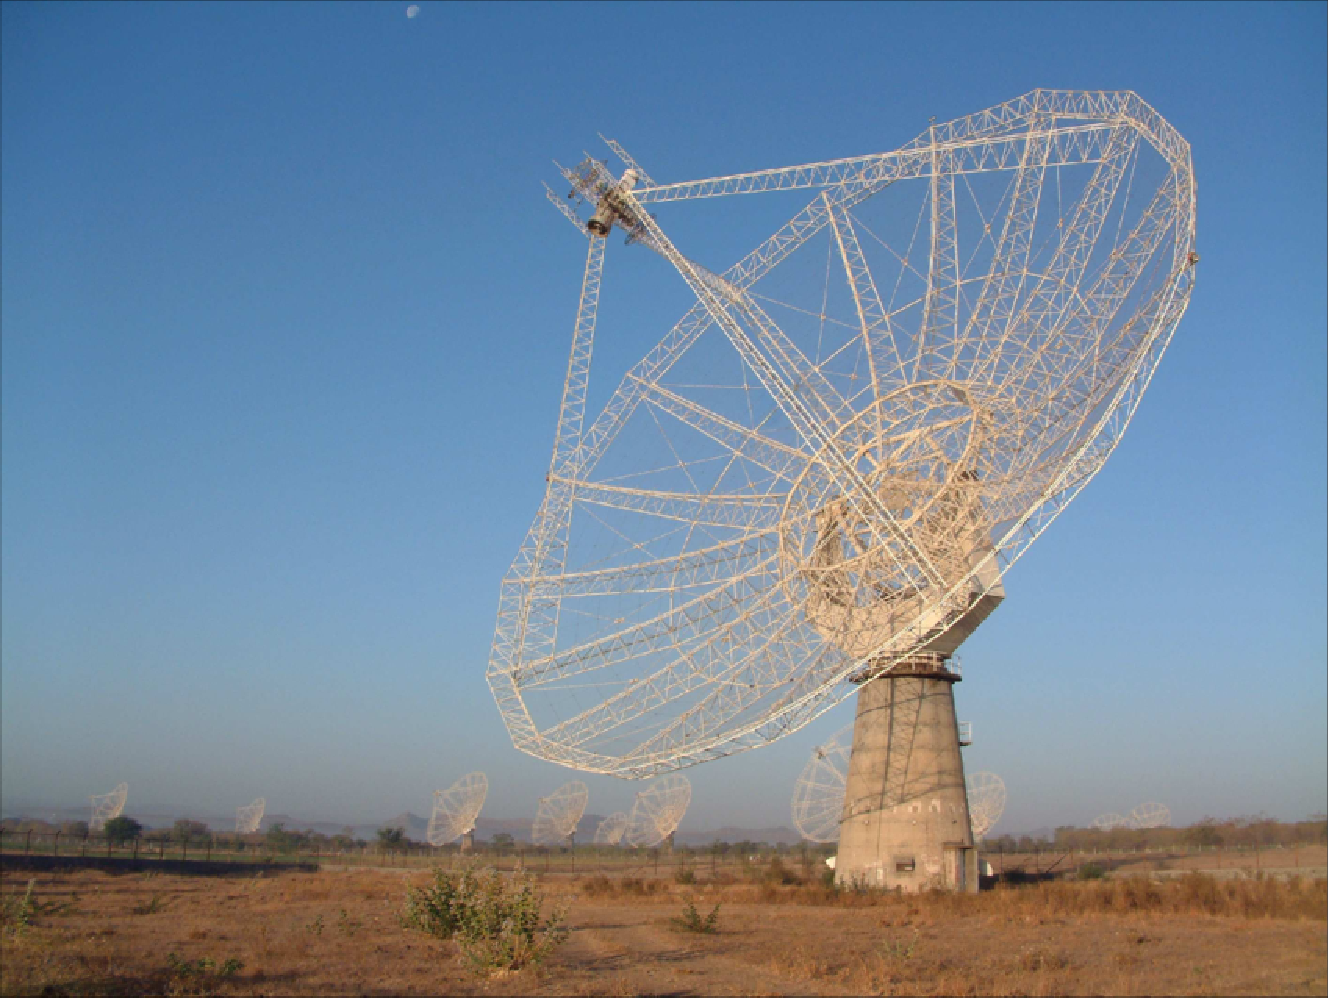
\includegraphics[width=0.44\textwidth]{pics/GMRT.pdf}} \;\;
    \scalebox{-1}[1]{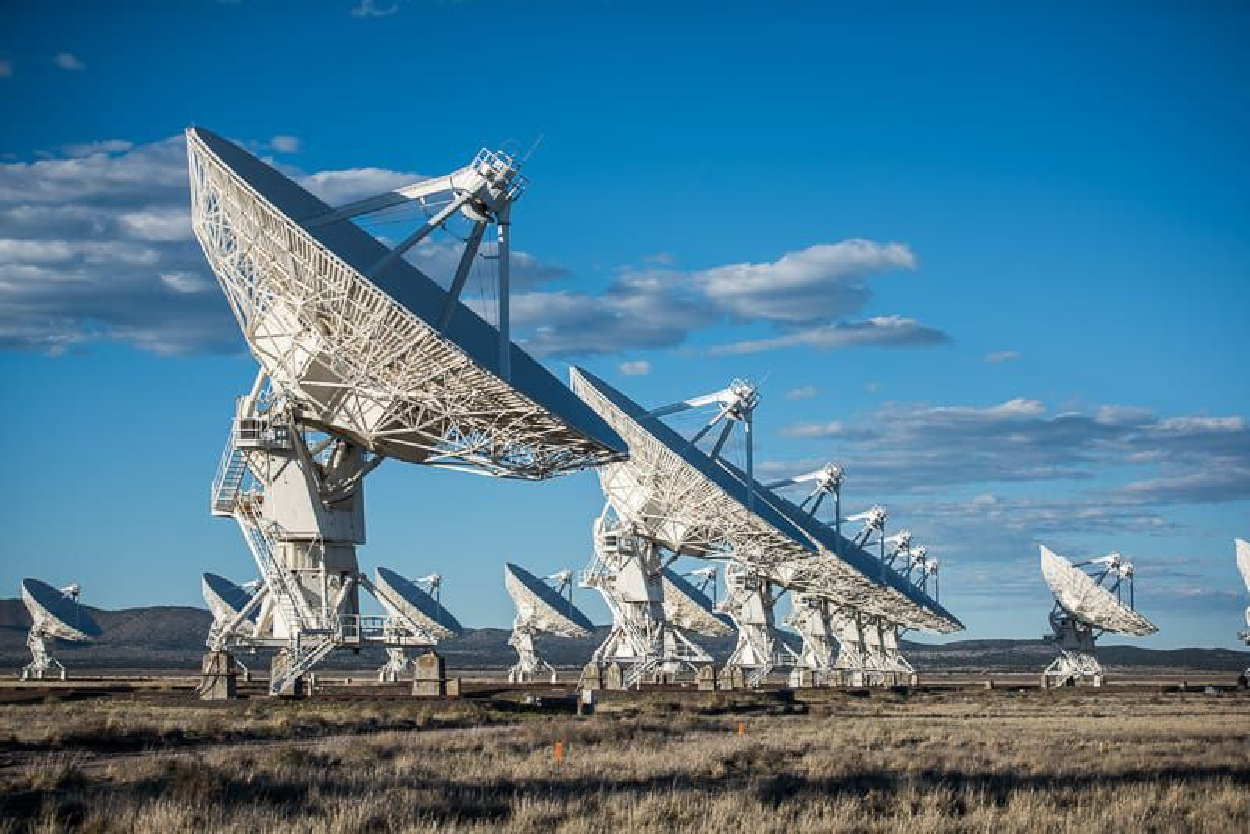
\includegraphics[width=0.5\textwidth]{pics/VLA.pdf}}
    \caption{Giant Metrewave Radio Telecope and Very Large Array\\
    (TGSS) 150 MHz / resolution $\ang{;;25}$ vs. (NVSS) 1.4 GHz / resolution $\ang{;;45}$}
\end{figure}

\newpage
\section{Introduction}
%cut-outs
\label{sec:source_catalogues}
% explain each of TGSS and NVSS

% motivation

% What's out there in the universe?

We consider matches between sources in TGSS (TIFR GMRT Sky Survey Alternative Data Release 1) and NVSS (NRAO VLA Sky Survey). A source in each of the surveys is a gaussian (blob) fitted over the raw data. To clarify, there are three layers at play: the real physical object that exists out in the universe, the raw photometric data detected by each of the Giant Metrewave Radio Telescope (TGSS) and Very Large Array (NVSS), and the sources as gaussians that are fit to the plane of raw data. Our task is to go from pairs of these sources (one in each survey) to partition the sky back into the original physical sources as best we can. \\

TGSS catalogues the entire radio sky north of $-\ang{53}$ DEC in 0.6 million sources at 147.5 MHz with resolution $\ang{;;25}$. From TGSS we extract for each source: the source name in IAU form TGSSADR JHHMMSS.S+DDMMSS, the RA and DEC position on the sky (in degrees), the lengths of the major and minor axes of the fitted gaussian (in arcseconds), the integrated (total) flux density (in milli-janskys: mJy) and peak flux (in mJy/beam), and the position angle (orientation on the sky) of the major axis (in degrees).\\

NVSS catalogues the entire radio sky north of $-\ang{40}$ DEC in 2 million sources at 1.4 GHz with resolution $\ang{;;45}$. From NVSS we extract for each source: the source name in IAU form NVSS JHHMMSS+DDMMSS, the RA and DEC position on the sky (in degrees), the lengths of the major and minor axes (in arcseconds), the peak flux (in mJy/beam, uncorrected), the position angle (in degrees), as well as the integrated and peak residual flux (in mJy and mJy/beam), the integrated polarised flux density (in mJy) with its Stokes Q and U linear polarisation brightnesses (in mJy) as of the source's centre.

% Cross-identification
\begin{figure}
    \centering
    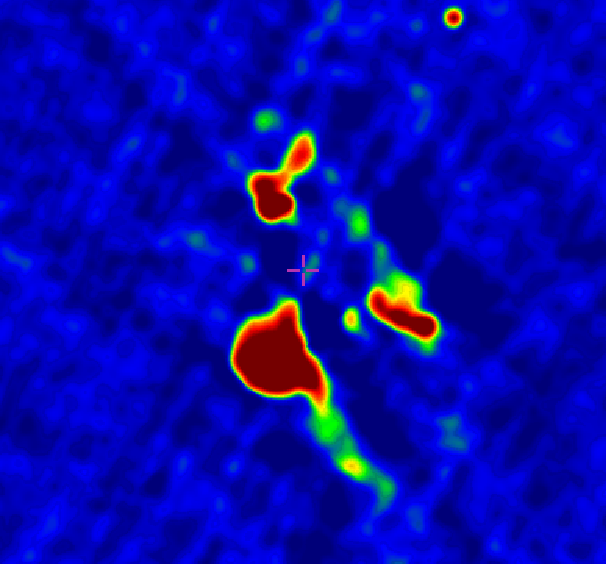
\includegraphics[width=0.48\textwidth]{pics/3c40t-cropped.pdf} \;\;
    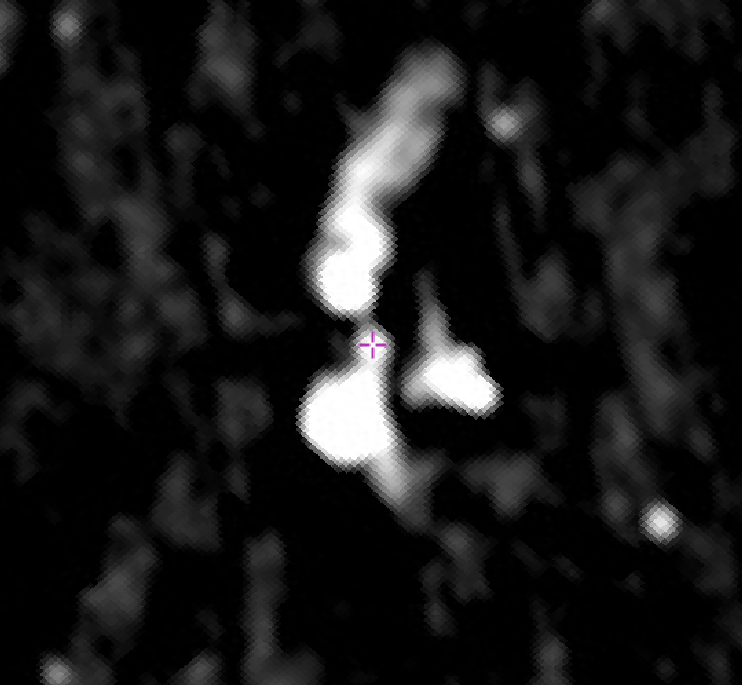
\includegraphics[width=0.48\textwidth]{pics/3c40n-cropped.pdf}
    \caption{Sources (blobs) of 3c40 in TGSS and NVSS}
    \label{fig:3c40}
\end{figure}

%  why is cross id non-trivial?


\newpage
\section{Positional matching}
Positional matching is determining matches purely based off the relative positions (RA and DEC) of each source on the sky. Assuming isotropy, this amounts to just considering the angular separation (geodesic distance on the celestial sphere) between their centres. For compact sources (tight, that subtend a small angle) this is a great filter as we'd scarcely expect two compact blobs on the sky degrees apart to have come from the same physical object. However, in radio, this is not a universal assumption as we have sources like the radio galaxy Centaurus A that cover about $\ang{8}$ on the sky (to the Moon's $\ang{0.5}$), or more commonly sources like 3c40 in figure~\ref{fig:3c40} that cover arcminutes. We take $\ang{;2;}$ as our separation limit when matching the entire sky, note that the expected number of matches grows as the square of this limit as the area of the disk of possible matches grows. We reject all matches beyond this limit, so we're at least missing direct matches for the degree sized objects on the sky. Whether partitioning can recover them remains to be seen.

\subsection{Positional matching results}
\label{sec:posmatch}
% explain plots and comparison

Initially, we consider matches of TGSS sources to NVSS sources over the entire sky that both surveys cover (north of $-\ang{40}$ DEC). In part, because we have a reference to the same being done recently in \citet{posmatchpaper}, albeit with some differences: \citet{posmatchpaper} uses a closer $\ang{;;30}$ separation limit and drops all non-unique matches. When we train a logistic regression classifier, we do so on a $\ang{20}\times\ang{20}$ patch of common southern sky and with a separation limit of $\ang{;10;}$.

% hist_angle
\begin{figure}[H]
    \centering
    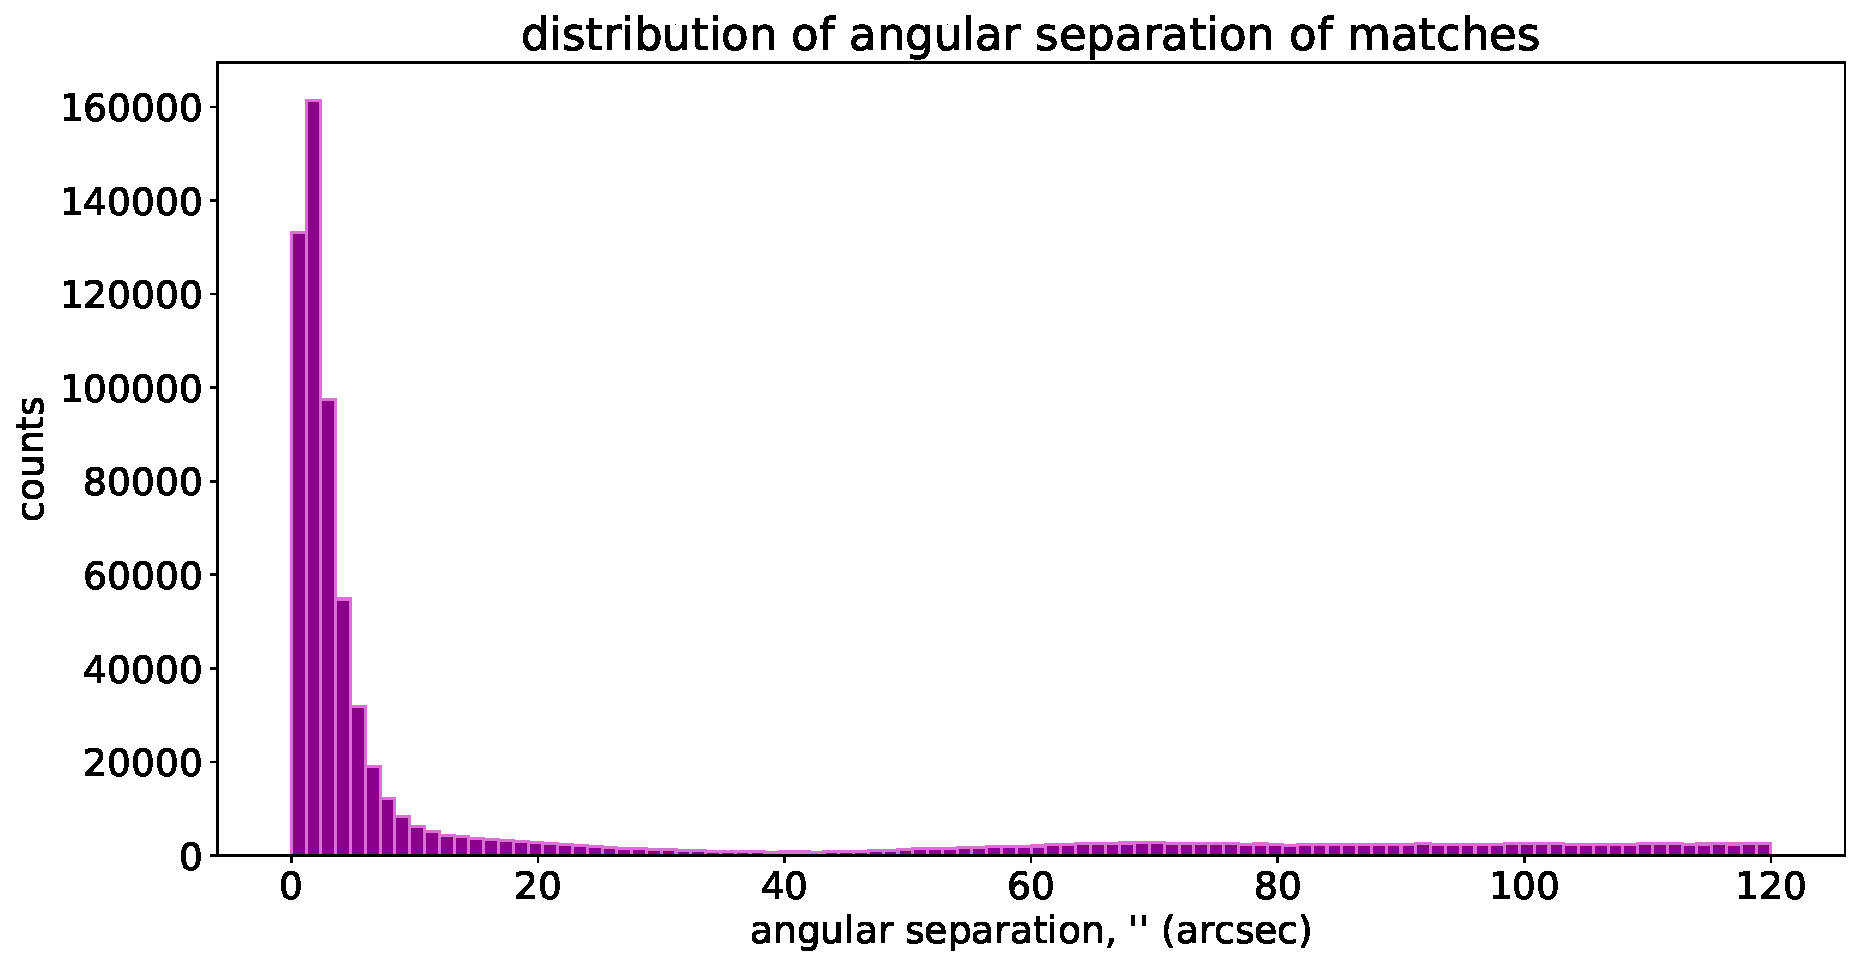
\includegraphics[width=\textwidth]{pics/hist_angle.pdf}
    \caption{Distribution of angular separation of positional matches TGSS-NVSS over entire common sky (north of $-\ang{40}$ DEC) for a separation limit of $\ang{;2;}$, note the bi-modality within this range into populations either side of $\ang{;;40}$.}
    \label{fig:hist_angle}
\end{figure}

See figure~\ref{fig:hist_angle} for the distribution of separations for matches (TGSS-NVSS) over the entire common sky. In total, we find over 720000 matches within $\ang{;2;}$ in a bi-modal distribution split either side of $\ang{;;40}$, with the vast majority of matches within $\ang{;;10}$. This bi-modality is hypothesised as being the result of two effects, geometric more than cosmological: actual matches between objects (\citet{tgss} estimates 94.4\% of TGSS sources have a NVSS counterpart within $\ang{;;45}$) and then the start of a long quadratic as the search window widens and collects more and more matches. That is, if we extended the search out to $\ang{180}$ we'd match the entire sky and we expect the curve to get there to be quadratic in the search radius. We'll use this cut at $\ang{;;40}$ to threshold (activate) the label of the match as it's the clearest distinction that positional matching returns. To be clear though, we have no reason to suspect all these matches within $\ang{;;40}$ to be between sources from the same physical object, but we do chose to train that that positional matching label.

\subsection{Catalogue of matches}
% pair T / N and making the catalogue
% Note: an exact definition of feature vectors and labels will follow in section~\ref{sec:napkin_intro_to_ml}, here we just consider them vaguely.
We construct a common catalogue of the positional matches of TGSS to NVSS over a $\ang{20}\times\ang{20}$ square patch of sky between $-\ang{35}\mathrm{RA}, \ang{149}\mathrm{DEC}$ and $-\ang{15}\mathrm{RA}, \ang{169}\mathrm{DEC}$ (i.e. centred on $-\ang{25}\mathrm{RA}, \ang{159}\mathrm{DEC}$), with a separation limit of $\ang{;10;}$. The choice of patch is arbitrary, testing shows no difference if the patch is moved (as long as it stays totally within the common sky), $-\ang{35}\mathrm{RA}, \ang{149}\mathrm{DEC}$ happens to be Canberra's latitude and longitude.\\

The main advantage of making a common catalogue is that we can add derived features from a combination of both sources.
See section~\ref{sec:source_catalogues} for details of each of the raw and fitted features from the source catalogues that we save into the common catalogue. The first of the derived features we add is separation. Later, we'll assume isotropy and remove the RA and DEC position values.
The disadvantage of making this common catalogue from positional matching is precisely that we must chose some separation limit and rule out degree sized objects, or create far too cumbersome a catalogue filled mostly with matches between unrelated compact sources far away from each other.
% This also allows us to impose isotropy and remove the RA and DEC values when we go to train, although they remain in the saved catalogue.\\
% The disadvantage to this approach is that we impose positional matching onto the dataset three times over: we only allow sources within a $\ang{20}$ patch, only allow matches within $\ang{;10;}$, and we label 1 any matches within $\ang{;;40}$. However, despite examples like Centaurus A, we argue that this can be treated as positional matching for compact sources, and that the loss of degree sized objects is worth it computationally.

\subsection{Spectral index}
The second derived feature that we can add is the spectral index, $\alpha$. The observed spectral index for a TGSS-NVSS match assumes the peak flux follows a power law of frequency, takes the ratio of sources, and re-arranges for the best guess at the exponent ($\alpha$) were the two sources the same object:
\begin{equation}
\label{eq:alpha}
\begin{split}
S_\nu &= \nu^\alpha \\
S_\mathrm{TGSS}/S_\mathrm{NVSS} &= (\nu_\mathrm{TGSS}/\nu_\mathrm{NVSS})^{\alpha_\mathrm{obs}} \\
\alpha_\mathrm{obs} &= \frac{\log(S_\mathrm{TGSS}/S_\mathrm{NVSS})}{\log(\nu_\mathrm{TGSS}/\nu_\mathrm{NVSS})}
\end{split}
\end{equation}
See figure~\ref{fig:hist_alpha_comparison} for the distribution of the observed spectral index of matches over the entire common sky, and a comparison of the same plot from \citet{posmatchpaper}. Note here a mistake (on my part) in that peak flux did not get corrected for beam size for either survey when calculating each match's spectral index. The main distribution appears roughly identical between plots, except for the fatter tails in ours with a right tail preference for higher peak fluxes. Unlike \citet{posmatchpaper}, we did not drop non-unique matches and had a larger separation limit and those must therefore allow matches with more diverse alpha values. This makes sense, the more non-unique matches we allow, the more different we'd expect the sources to be and so the more diverse alpha values we'd allow. That the right tail preferences higher peak fluxes from TGSS follows from higher fluxes allowing stronger ratios within the spectral index formula, see equation~\ref{eq:alpha}.\\

% hist_alpha
\begin{figure}[H]
    \centering
    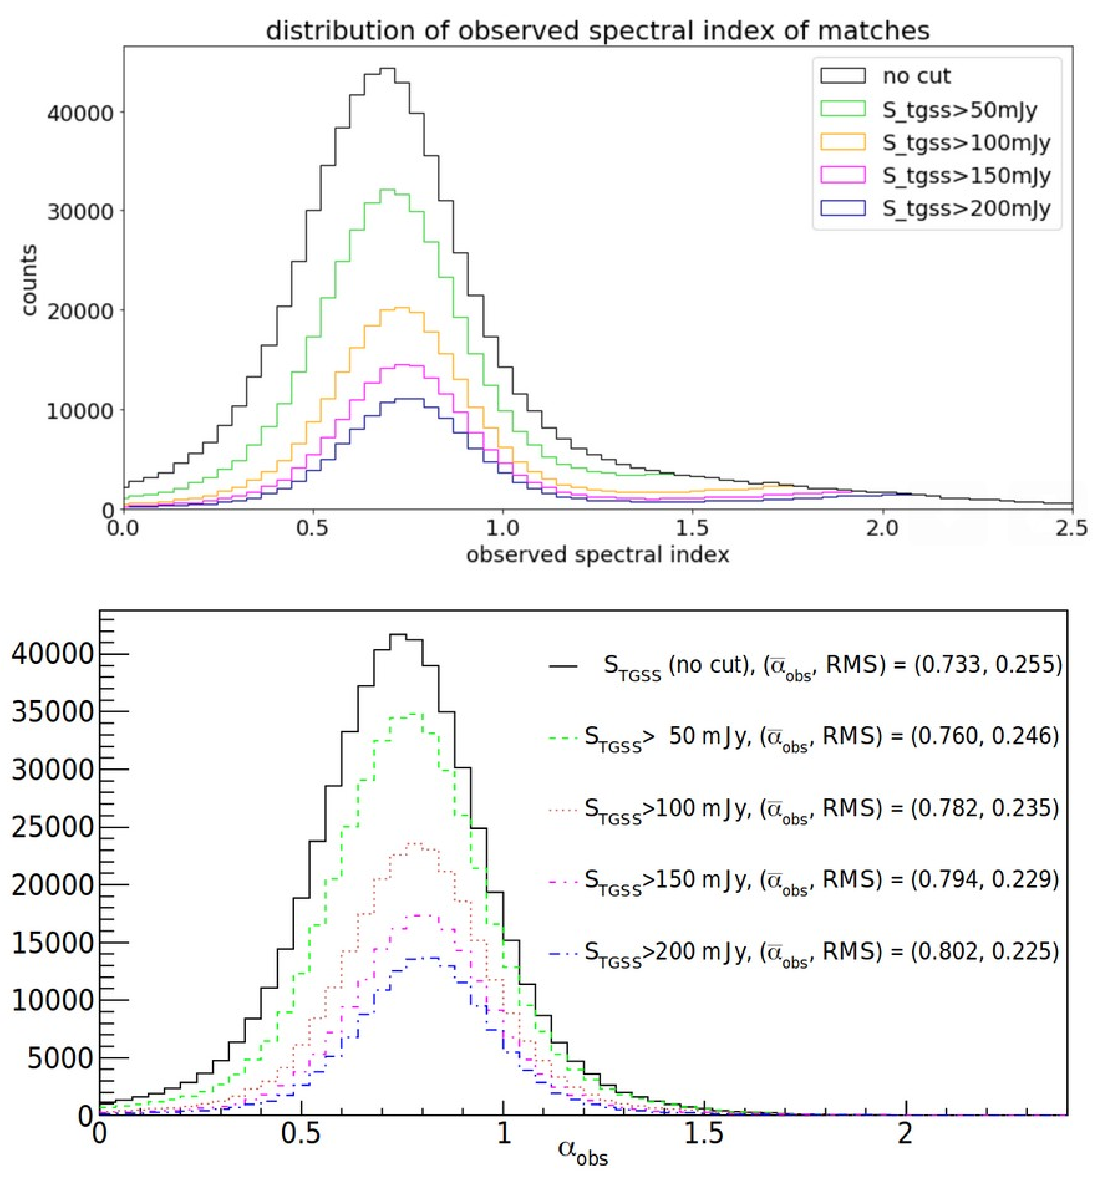
\includegraphics[width=\textwidth]{pics/hist_alpha_comparison-cropped.pdf}
    \caption{Spectral index $\alpha$ of positional matches over sky comparison to \citet{posmatchpaper}, caution: image used without permission. Note the fatter tails of our matching and the right tail preference for higher peak fluxes.}
    \label{fig:hist_alpha_comparison}
\end{figure}

The last derived feature was the logarithm of the various flux features as in section~\ref{sec:source_catalogues}, we added this only later in an input step, it isn't saved into the created catalogues. This is a common technique for treating the large range that fluxes can fall over.
% Note that unlike the other two derived features (separation and spectral index) this doesn't combine catalogues.

\newpage
\section{Logistic regression}
Having recreated existing positional matching results, we now return to the central problem of cross-identification to find physical objects. With our common catalogue of TGSS to NVSS positional matches, we choose to approach this problem as a binary classification task. Given a positional match, tell whether the sources come from the same physical object. Moreover, we can train an automated classifier to perform this task.\\

It's worth noting that this is not the only way to approach cross-identification, it doesn't even need to be binary classification. We could instead aim to train a predictor to take in any TGSS source and return the best match in NVSS, or take in a list of sources and return the likelihood of them all coming from the same object, or any number more of variations on the theme of cross-identification. We chose the binary classification given a pair of sources as it can work directly off of the positional matching catalogue already made and since it's is generally easier.

\subsection{A napkin-sized introduction to machine learning}
\label{sec:napkin_intro_to_ml}
Supervised machine learning considers a function, $f: X \rightarrow Y$
\begin{itemize}
    \item[$f$] is the function, called the classifier/predictor
    \item[$X$] is the input real-valued feature vectors from some space $\mathbb{R}^D$, where each component is called a feature
    \item[$Y$] is the output predictions to be compared against labels (of a similar type), predictions/labels are not necessarily real-valued scalars and decisions may need to be forced to transform predictions to the form of the labels
\end{itemize}
And we are interested in how the function operates on data: known inputs and their corresponding labels, i.e. $\text{dataset} = \{(\vec{x_1},\hat{y_1}), \ldots, (\vec{x_N},\hat{y_N})\}$. Where a distinction between the initial form of the predictions and form of the labels. Here, $\hat{y_i}$ is the known label associated with a feature vector $\vec{x_i}$, and we might call the prediction $f(\vec{x_i}) = y_i$. Alternatively, we can collapse the decision processes into the function and assume that prediction and labels are directly comparable.\\

Three related algorithms, all called machine learning, concern this function:
\begin{itemize}
    \item[(1)] training: optimising the function against training data
    \item[(2)] testing/prediction: evaluating the function on other, testing data
    \item[(3)] hyperparameter tuning/model selection: changing the other (non-feature) arguments and the form of the function and the training (e.g. changing the regulariser $\lambda$, see definition of cost below)
\end{itemize}

Training is optimising some objective for the function. With labels, this objective is often to minimise a cost function. Here, we consider cost functions of the form: the average of some loss function over the training data plus a regularising term with argument $\lambda$ (a hyperparameter). Loss functions are a metric between a prediction compared to a label, $\text{loss} = l(\hat{y_i},f(\vec{x_i}))$. See section~\ref{sec:loss} for more about loss. An example cost function would be $\text{avg loss} + \lambda\,\norm{\vec{\theta}\,}^2$, which would penalise models that strongly weighted lots of features. These three terms are very similar but operate on different scales, loss is at a particular data point, cost is over the whole training dataset, and the objective is more generalised goal of the training process (which here is to minimise the cost function).\\

Logistic regression is when the function is of the form:
\begin{equation}
\begin{split}
    f(\vec{x}\,) &= \sigma(\vec{\theta}\cdot\vec{x}+\theta_0) \\
    \sigma(x) &= \frac{1}{1+e^{-x}}       
\end{split}
\end{equation}
Where $\sigma$ is the logistic sigmoid, $\vec{\theta}$ the weights, and $\theta_0$ the bias. Compare to linear regression with $g(\vec{x}\,) = \vec{\theta}\cdot\vec{x}+\theta_0$. One can think that the function is really $f(x;\vec{\theta},\theta_0)$ and that training is adjusting these weight/bias arguments. Because logistic regression evaluates the feature vector all at once, we put it in a general class of so called linear classifiers, despite the fact that with the sigmoid it can learn non-linear features.

\subsection{Feature vectors and labels}
In the language of the previous section, we set up a logistic regression binary classifier to take in feature vectors of the common catalogue and return the likelihood of a match being real. To cut down the size of the problem, from here on we consider the common catalogue of the $\ang{20}$ patch with separation limit $\ang{;10;}$, rather than the entire shared sky.\\

Formally, translating raw data (z), in whatever form, through a feature map ($\phi$) into real-valued feature vectors ($\vec{x}$\,) is the work of a `domain expert'. In our case, all of the data in the common catalogue is already numerical (except the source names). For our feature map, we drop the RA and DEC positions and add in logarithm values of the flux and flux densities but otherwise don't alter the catalogue. In a sense, the real domain expertise came much earlier in the construction of TGSS and NVSS from truly raw photometric/geometric data. Also note that logistic regression generally assumes that all the features have been normalised, which our haven't, and binary classification generally assumes that the labelled population sizes are roughly equal, which our are (at 63\% negative to 37\% positive).\\

Finding labels and justifying them is the critical obstacle to supervised machine learning. We use the results from positional matching, in particular figure~\ref{fig:hist_angle}, to label all matches with separation less than $\ang{;;40}$ as a positive match, and all those with separation greater as a negative match. This is by the arguments in section~\ref{sec:posmatch}, in particular the observation of the distinct population of separations less than $\ang{;;40}$. We write an explicit score function for this labelling, which sets separation 0 to score 1 and then linearly decreases to 0 at and beyond the threshold of $\ang{;;40}$. See figure~\ref{fig:patch_scores_dist} for a plot of these scores over the patch.
% patch_scores_dist
\begin{figure}[H]
    \centering
    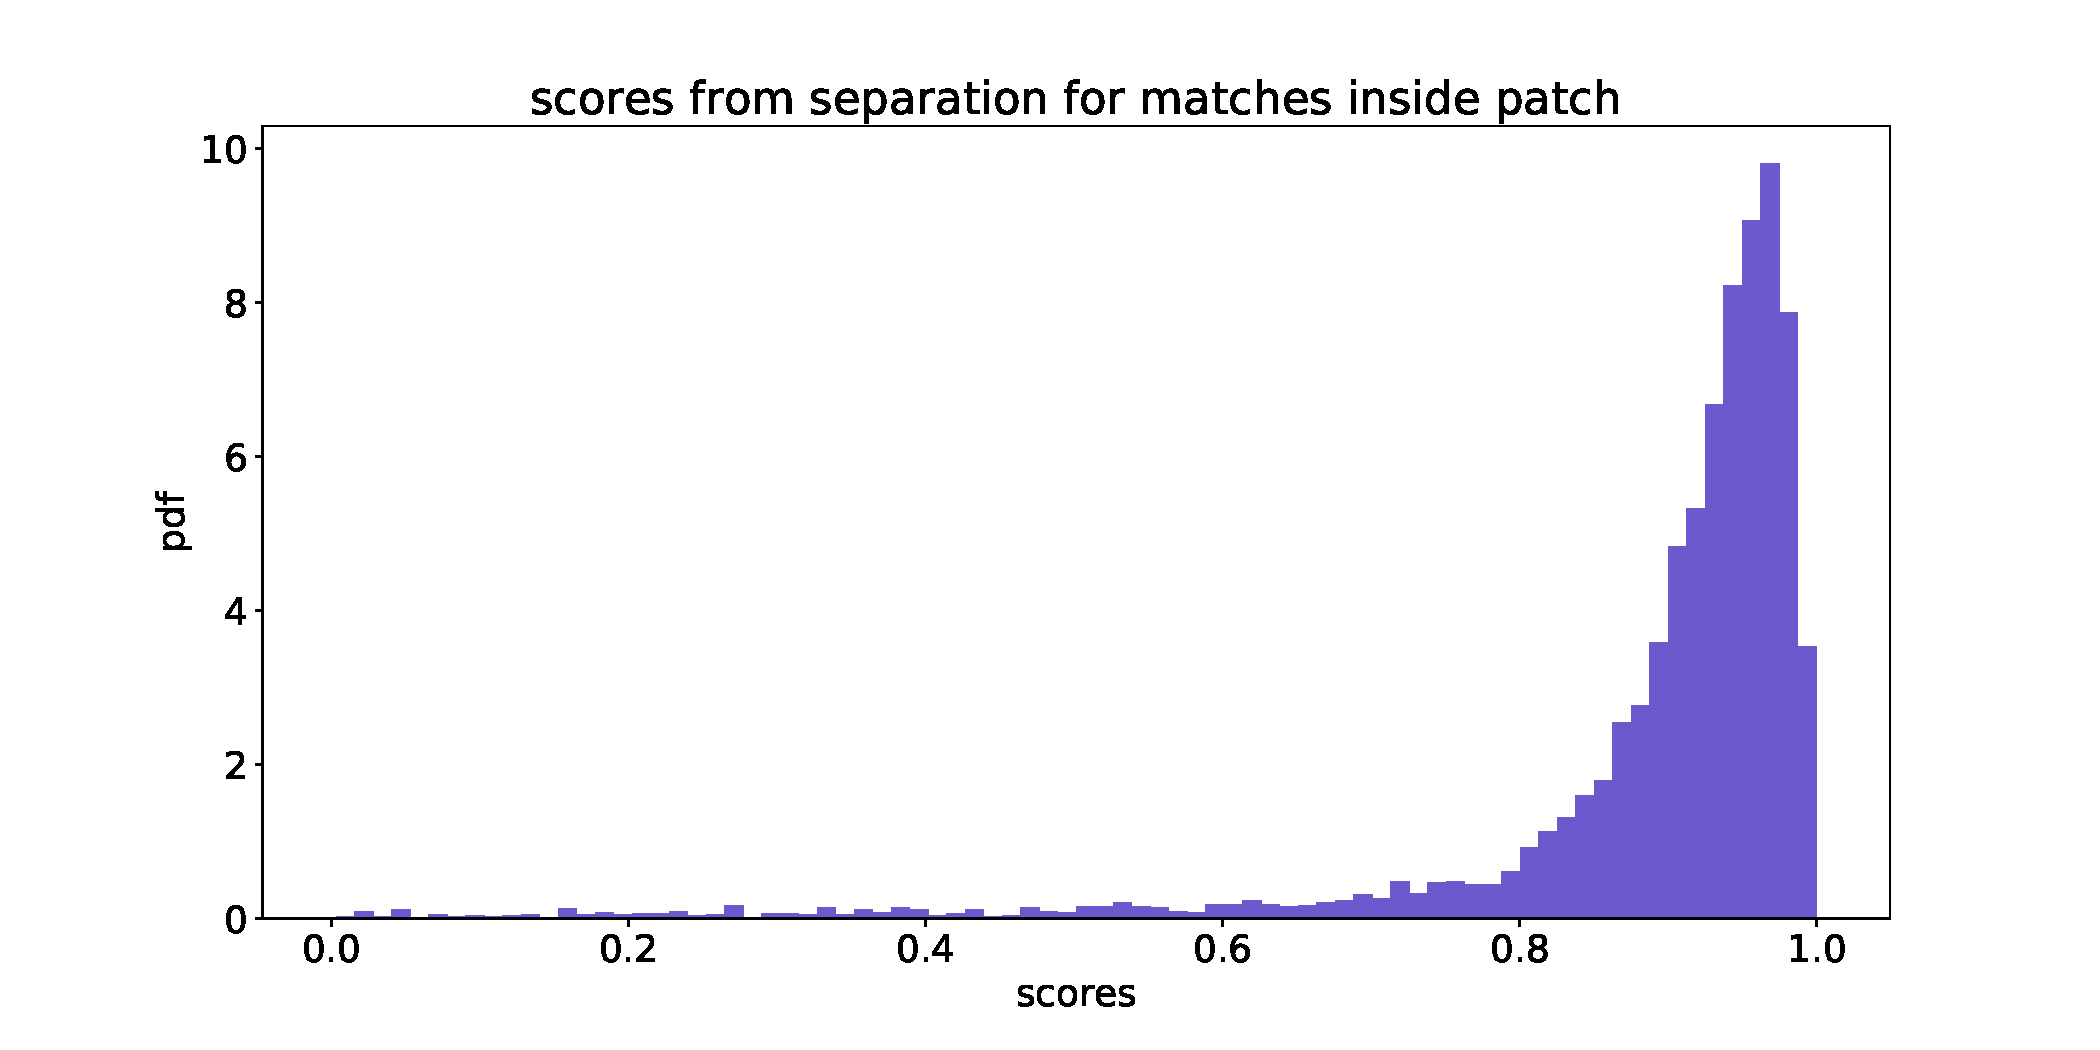
\includegraphics[width=\textwidth]{pics/patch_scores_dist.pdf}
    \caption{Separation based score with threshold at $\ang{;;40}$, distribution for all matches in patch. Compare to figure~\ref{fig:hist_angle}.}
    \label{fig:patch_scores_dist}
\end{figure}

During research, we also created some other explicit score functions for general matches than the separation scorer. Variations included: checking if a match was in the catalogue, using the spectral index histogram as a pdf, and weighted combinations thereof against the separation score. These hand-made score functions did not produce nice results and were left behind for logistic regression.

\newpage
\subsection{Loss}
\label{sec:loss}
%  |      | l
%  | 1    | __
We use the binary cross-entropy (BCE) of labels against predictions as our loss term. Information theoretically, this represents the expected information gain ($-\log_2{\mathrm{(prob)}}$) over the labels from observing the correct prediction, or the expected coding length (in bits) of the labels given optimised lengths for the predictions. Note that the use of expected value instead of average here is improper. This is closely related to the Kullback-Leibler Divergence between the label and prediction distributions, $D_{KL}(\mathrm{labels}\,\rvert\rvert\,\mathrm{predictions})$. Being binary means that the labels only take on values $y_n = 0 \mathrm{\;or\;} 1$, and let $f_n$ be the corresponding prediction to a particular label, with n observations going from 1 to the sample size N.
\begin{equation}
\begin{split}
    H_f(y) = \mathbb{E}_y [- \log_2(f)] = - \sum_{i} (y_i \log_2(f_i))
    \stackrel{*}{=} - (y \log_2(f) + (1-y) \log_2(1-f)) \\
    \therefore\; \mathrm{average\; loss} = \mathbb{E}_n [{H_f}_n(y_n)] = -\frac{1}{N} \sum_{n=1}^N (y_n \log_2(f_n) + (1-y_n) \log_2(1-f_n))    
\end{split}
\end{equation}
Note the trick in the last equality of the first line (*) that uses the binary label to explicitly write out both cases. And that cross entropy can also be notated (confusing it with joint entropy) as $H(y,f)$. Using this we can derive the average loss, which here equals the objective ($\mathrm{average\; loss} + \lambda \norm{w}^2$) as we've set a null regulariser ($\lambda=0$). Terms are confusing and often vague, but here the loss function is BCE, the cost function is average loss plus regulariser, which is also the objective function here. Since our objective function is just a cost function we'll drop the term `cost' and call it the objective, but note that in general the objective does not have to be a loss-based cost function. This form of the average loss is the negative of the log-likelihood, so minimising this average loss is the same as maximising the likelihood of successfully observing the labels.\\

During training, the algorithm is told to minimise the objective (the above average loss) by gradient-decent. Again, here the regulariser (the penalty to over-fitted, complex models) is set null so average loss is cost is objective. In pytorch \citep{torch} this is performed by backpropagation through automatic differentiation. Backpropagation is essentially the chain rule of differentiation except instead of applied to the entire function symbolically, applied along each sub-calculation throughout the function. This means that evaluating the function and evaluating its derivative have the same complexity since they follow the same set of sub-calculations. Once you have the gradient, you take a tiny step in the opposite direction and repeat.
% (recalling that the gradient vector points at the steepest uphill section and we want to minimise). Given a nowhere constant, differentiable (smooth is better) function over a compact domain this process will reach a local minimum or the boundary. Noting that odd behaviour can happen around a minimum due to the length of the step taken, one may end up oscillating about the minimum.

\newpage
\subsection{Logistic regression results}
% explain f, g, and h  and the three types of predictors
% plot prediction histograms with labelled populations, two humps



{\large
\begin{equation}
    \label{eq:predictionprocess}
    z \xrightarrow{\mathmakebox[3em]{\phi}} \bigg\rvert \; x \xrightarrow{\mathmakebox[3em]{score}} \mathbb{R} \xrightarrow{\mathmakebox[3em]{\sigma}} [0,1] \xrightarrow{\mathmakebox[3em]{activation}} \{0,1\}
\end{equation}}

It is worth (informally) remarking here that actually running logistic regression, after feature vectors and labels were all set up, went particularly fast leading to the remark: `and I thought machine learning was difficult'! In this lies what I identify as the TV Chef Problem, where if all the ingredients are prepared off-screen, the problem looks easy. However, this hides that sourcing and preparing those ingredients (translating data to feature vectors and deciding on labels), as well as determining if you've even got the right recipe (choosing models and tuning hyper-parameters), to actually serving the meal (interpreting results) is where the real difficulty and ambiguity lies. Watching the TV Chef is effortless, but answering: `is this meal right?' can be really hard.

% torch_lr_weights
\begin{figure}[H]
    \centering
    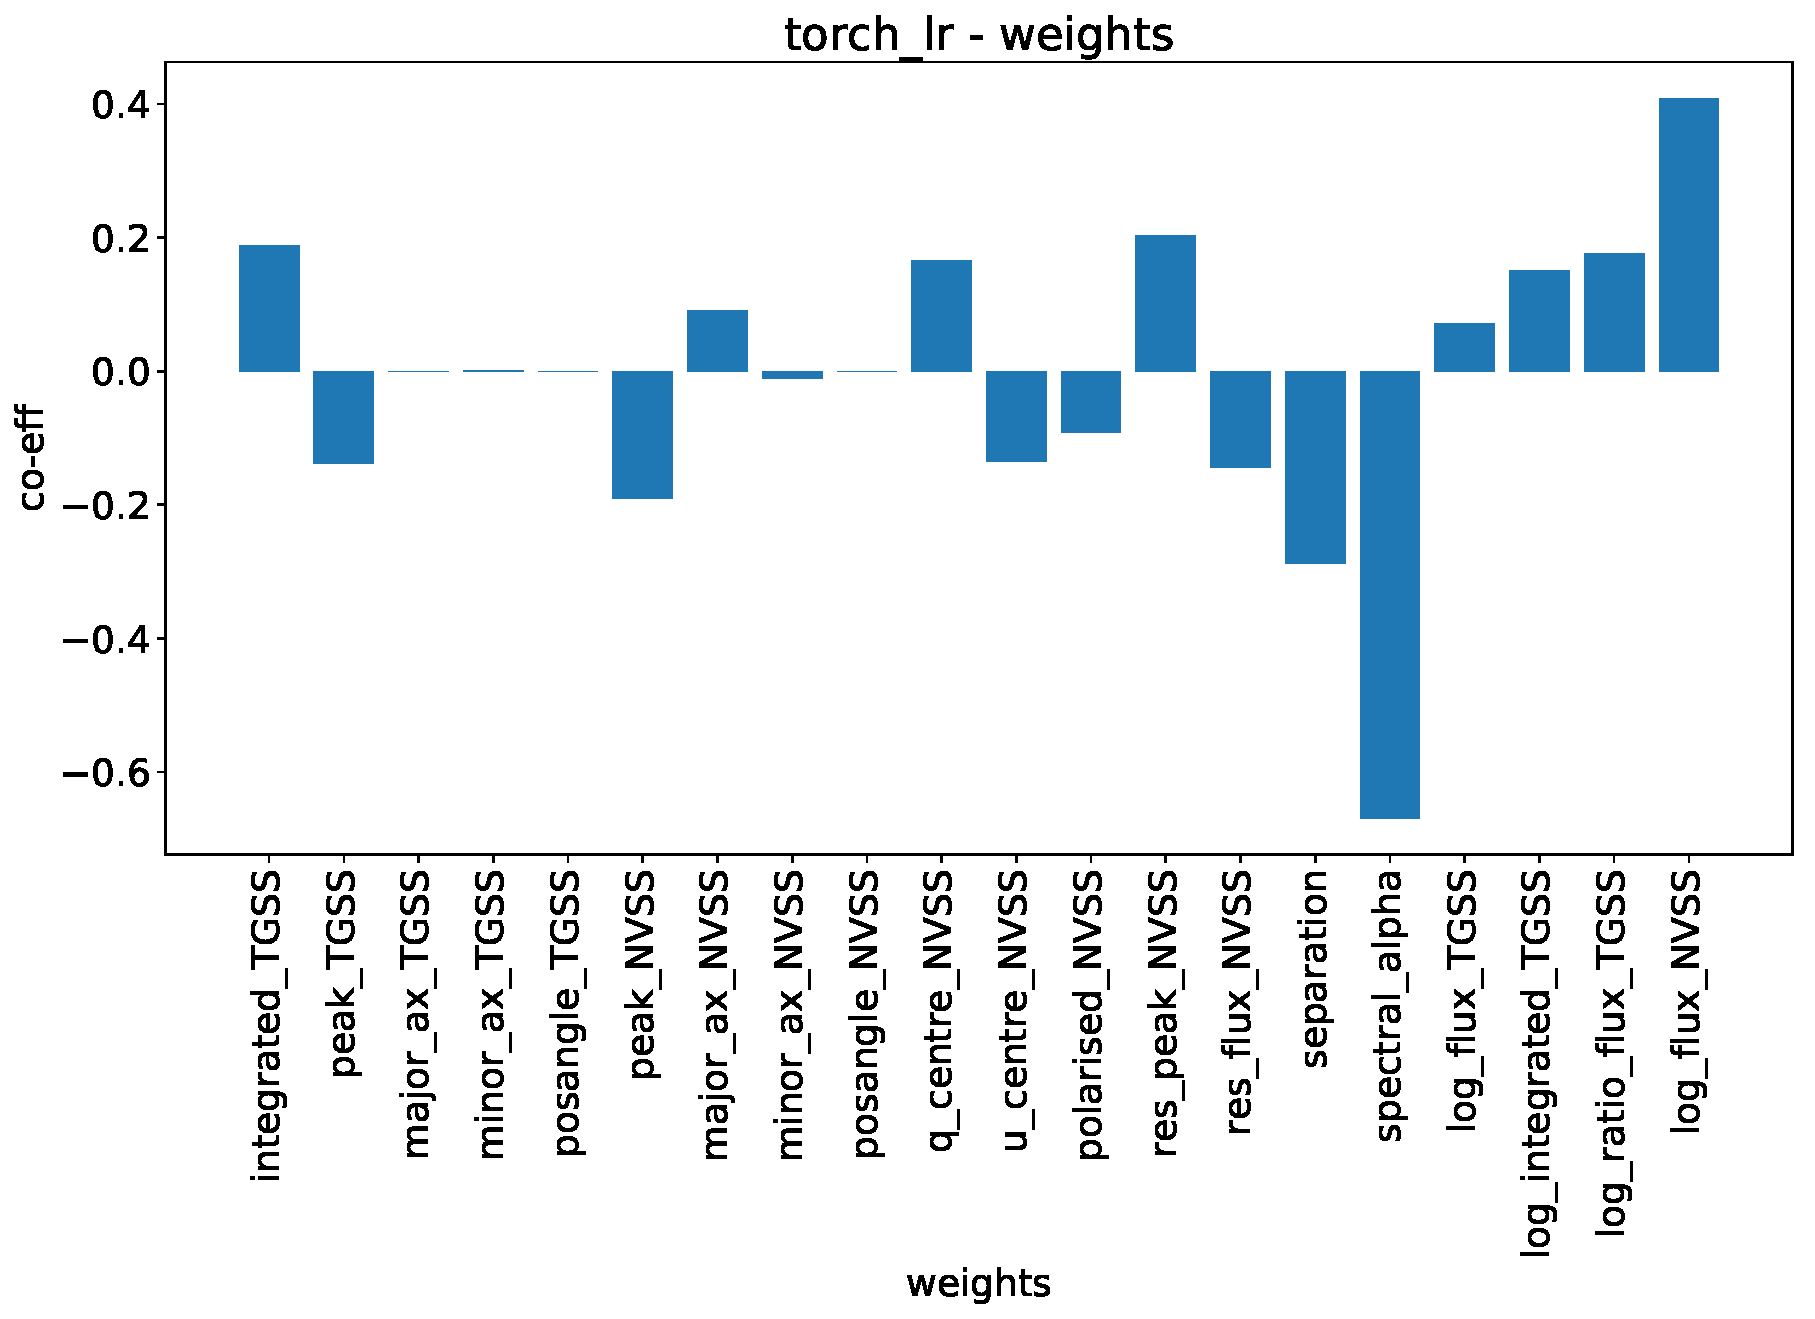
\includegraphics[width=\textwidth]{pics/torch_lr_weights.pdf}
    \caption{Weights in logistic regression model}
    \label{fig:torch_lr_weights}
\end{figure}

% torch_lr_weights_nosep
\begin{figure}[H]
    \centering
    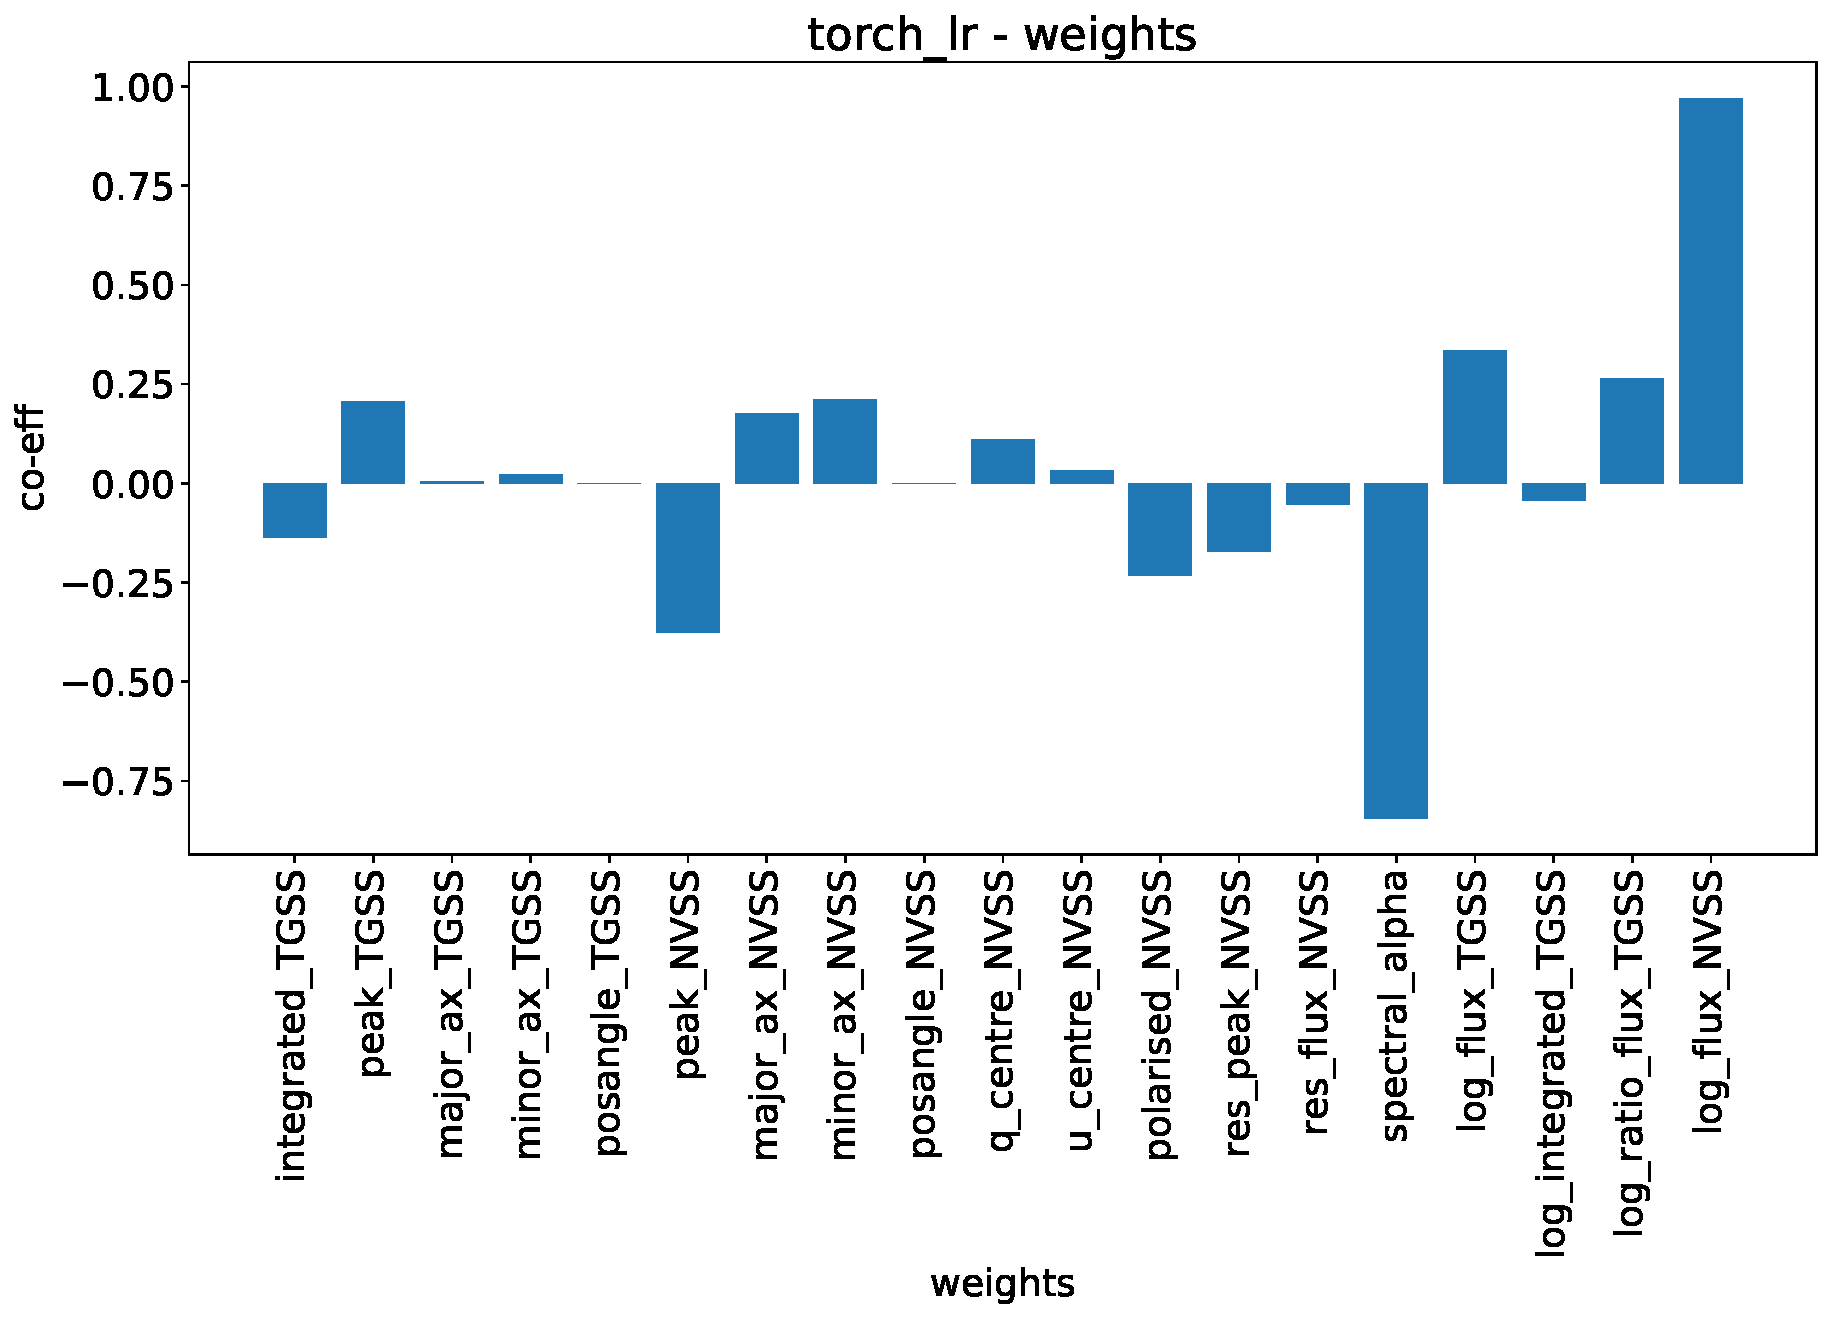
\includegraphics[width=\textwidth]{pics/torch_lr_weights_nosep.pdf}
    \caption{Weights in logistic regression model with separation removed}
    \label{fig:torch_lr_weights_nosep}
\end{figure}

\begin{table}[ht]
\centering
\resizebox{\textwidth}{!}{%
\begin{tabular}{rl|c|c|c}
 &  & \multicolumn{1}{r|}{accuracy} & \multicolumn{1}{r|}{precision} & \multicolumn{1}{r}{recall} \\ \hline
\multirow{2}{*}{\begin{tabular}[c]{@{}r@{}}pytorch: all\\ features\end{tabular}} & over patch catalogue & 75.7 & 42.3 & 90.2 \\ \cline{2-5} 
 & over manual labels & 80.0 & 80.0 & 100 \\ \hline
\multirow{2}{*}{\begin{tabular}[c]{@{}r@{}}pytorch: no\\ separation\end{tabular}} & over patch catalogue & 70.3 & 36.9 & 88.2 \\ \cline{2-5} 
 & over manual labels & 80.0 & 80.0 & 100 \\ \hline
\multirow{2}{*}{scikit-learn} & over patch catalogue & 97.4 & 90.2 & 96.3 \\ \cline{2-5} 
 & over manual labels & 82.5 & 100 & 78.1
\end{tabular}%
}
\caption{Accuracy percentages for logistic regressions: with all features or with all minus separation, and over the patch with positional matching labels or over manual labels. Note that recall is heavily preferenced against precision, so the classifier says a lot of matches are true, including most of the labelled true ones, but far more labelled false ones. See appendix~\ref{app:sklearn} for scikit-learn information.}
\label{tab:accuracy}
\end{table}

% torch_lr_predictions
\begin{figure}[H]
    \centering
    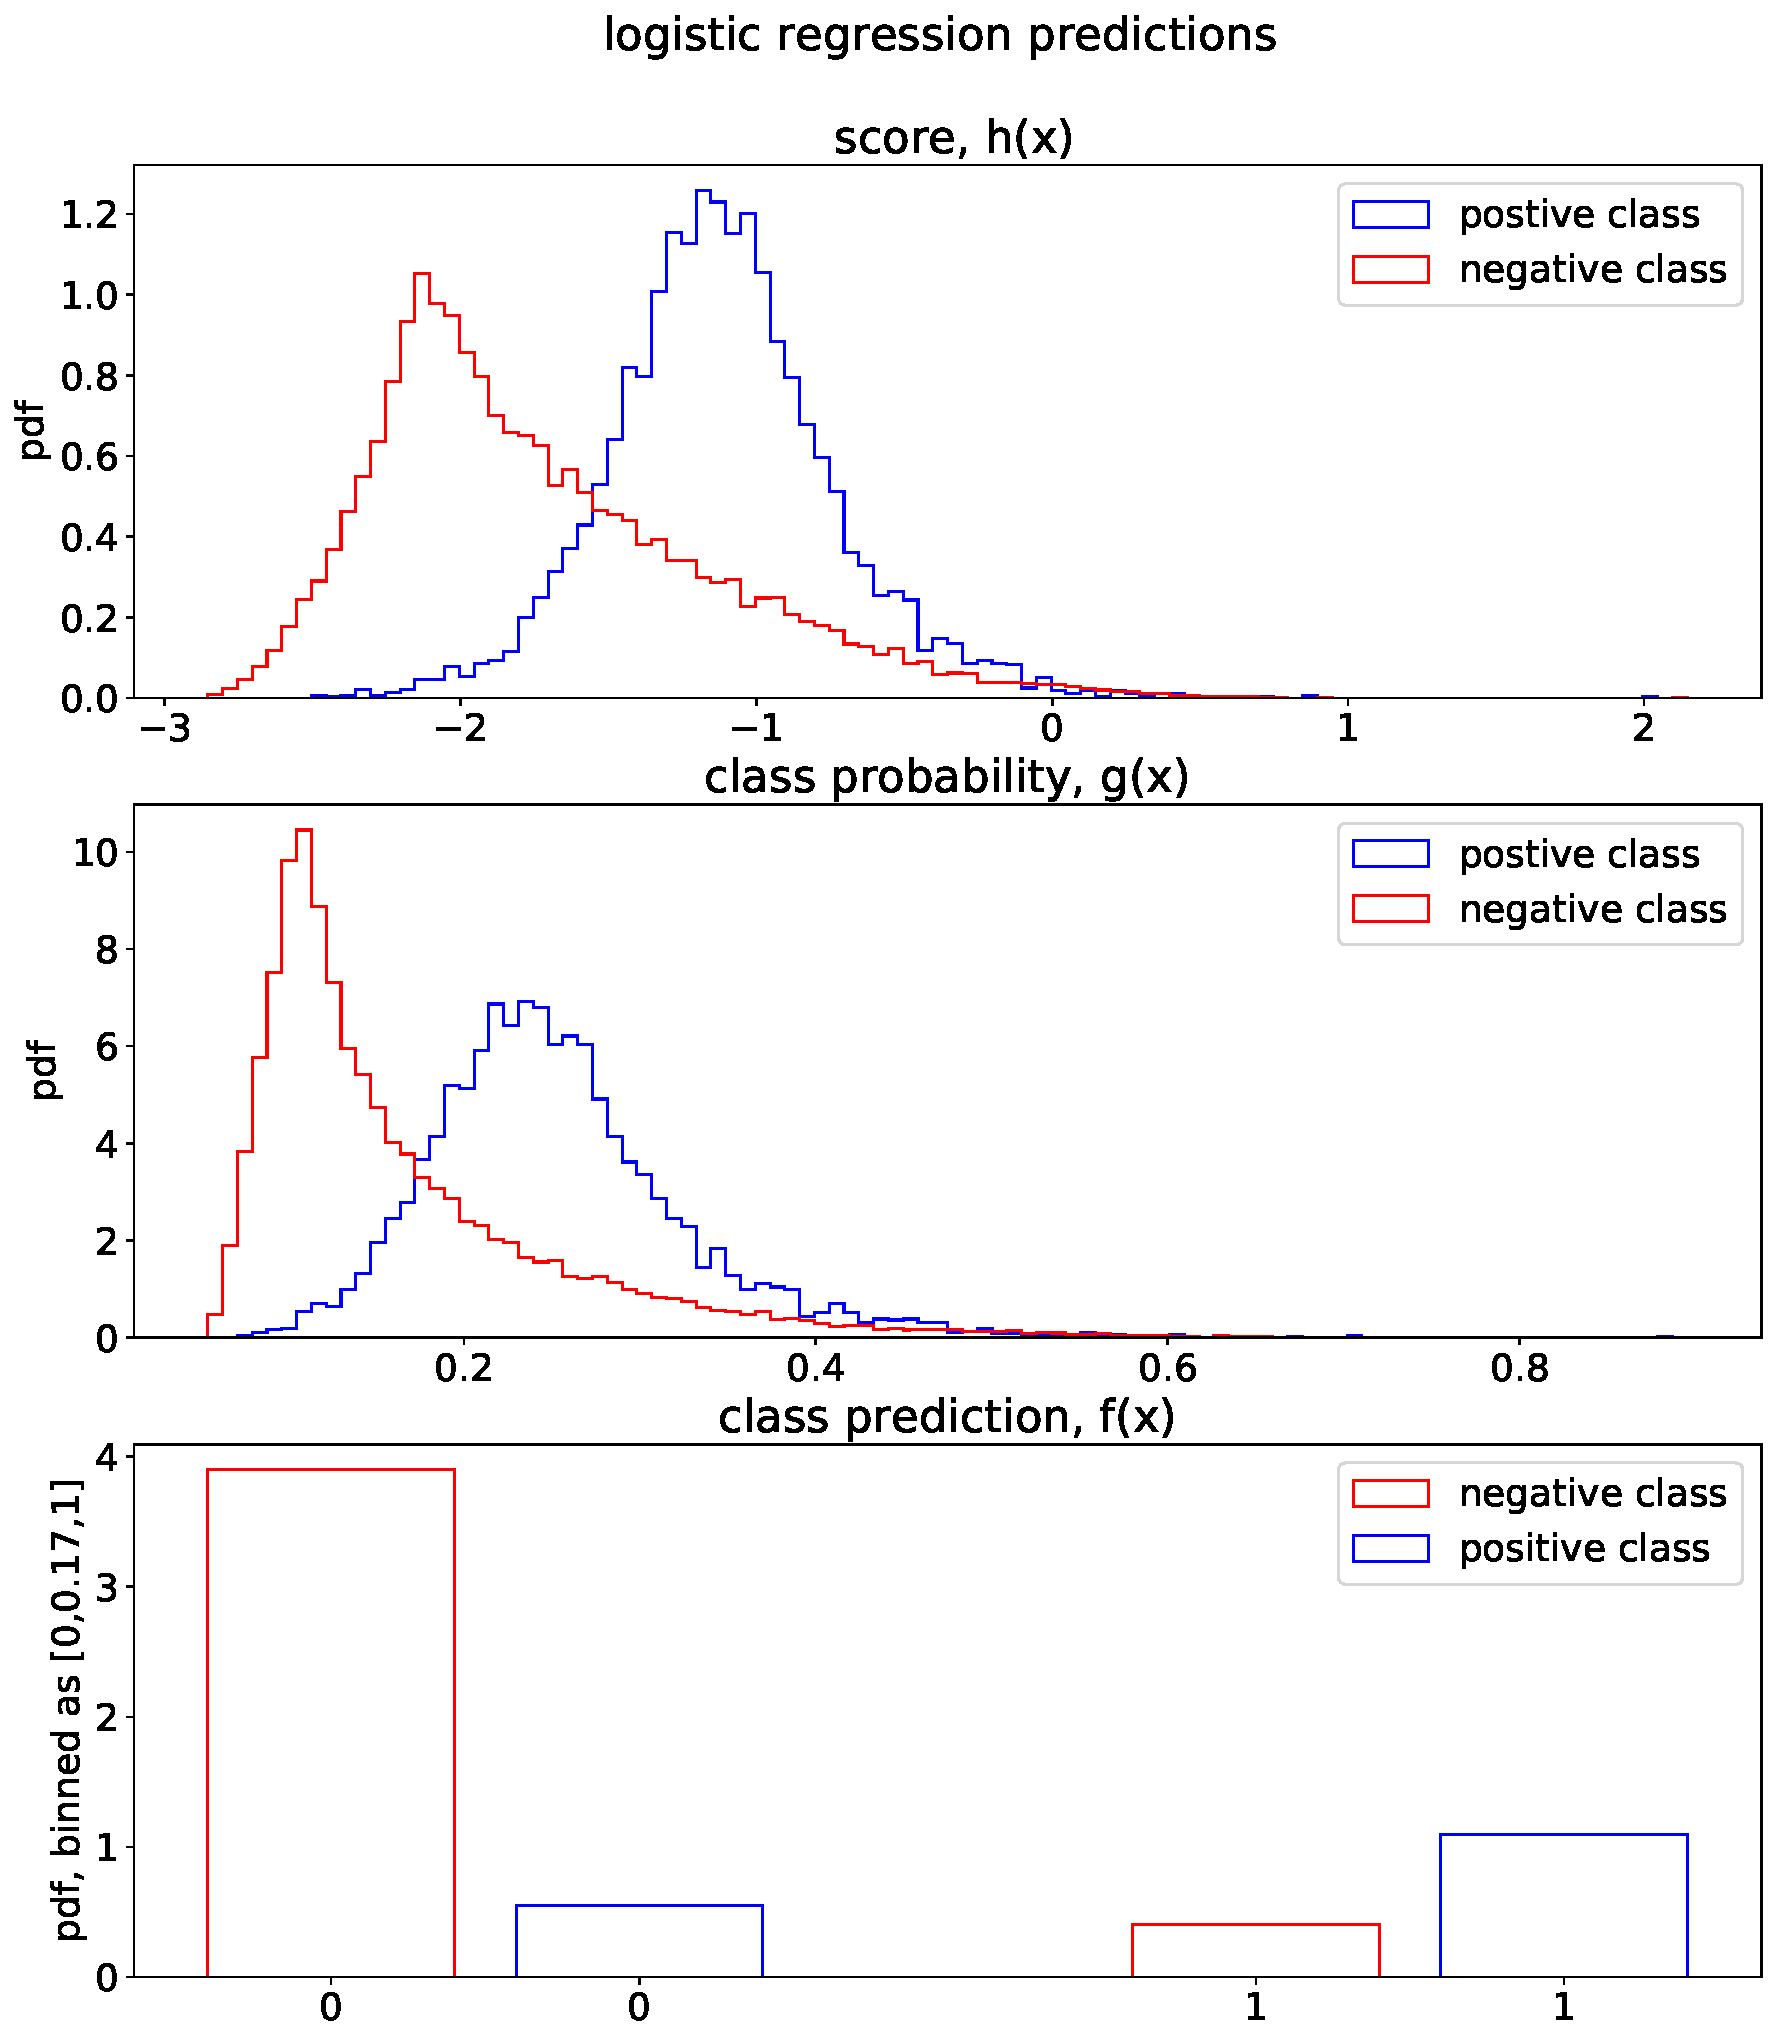
\includegraphics[width=\textwidth]{pics/torch_lr_predictions.pdf}
    \caption{Three related types of predictors for the binary classifier: the raw score over the whole real axis, the class probability within $[0,1]$, and the predicted class (0 or 1), here splitting where the two labelled populations meet at 0.17}
    \label{fig:fghpredictions}
\end{figure}


\subsection{Naive partitioning using classifier}
% explain how to get from log reg to object list

% torch_lr_partition, pretty snowflake picture
\begin{figure}[H]
    \centering
    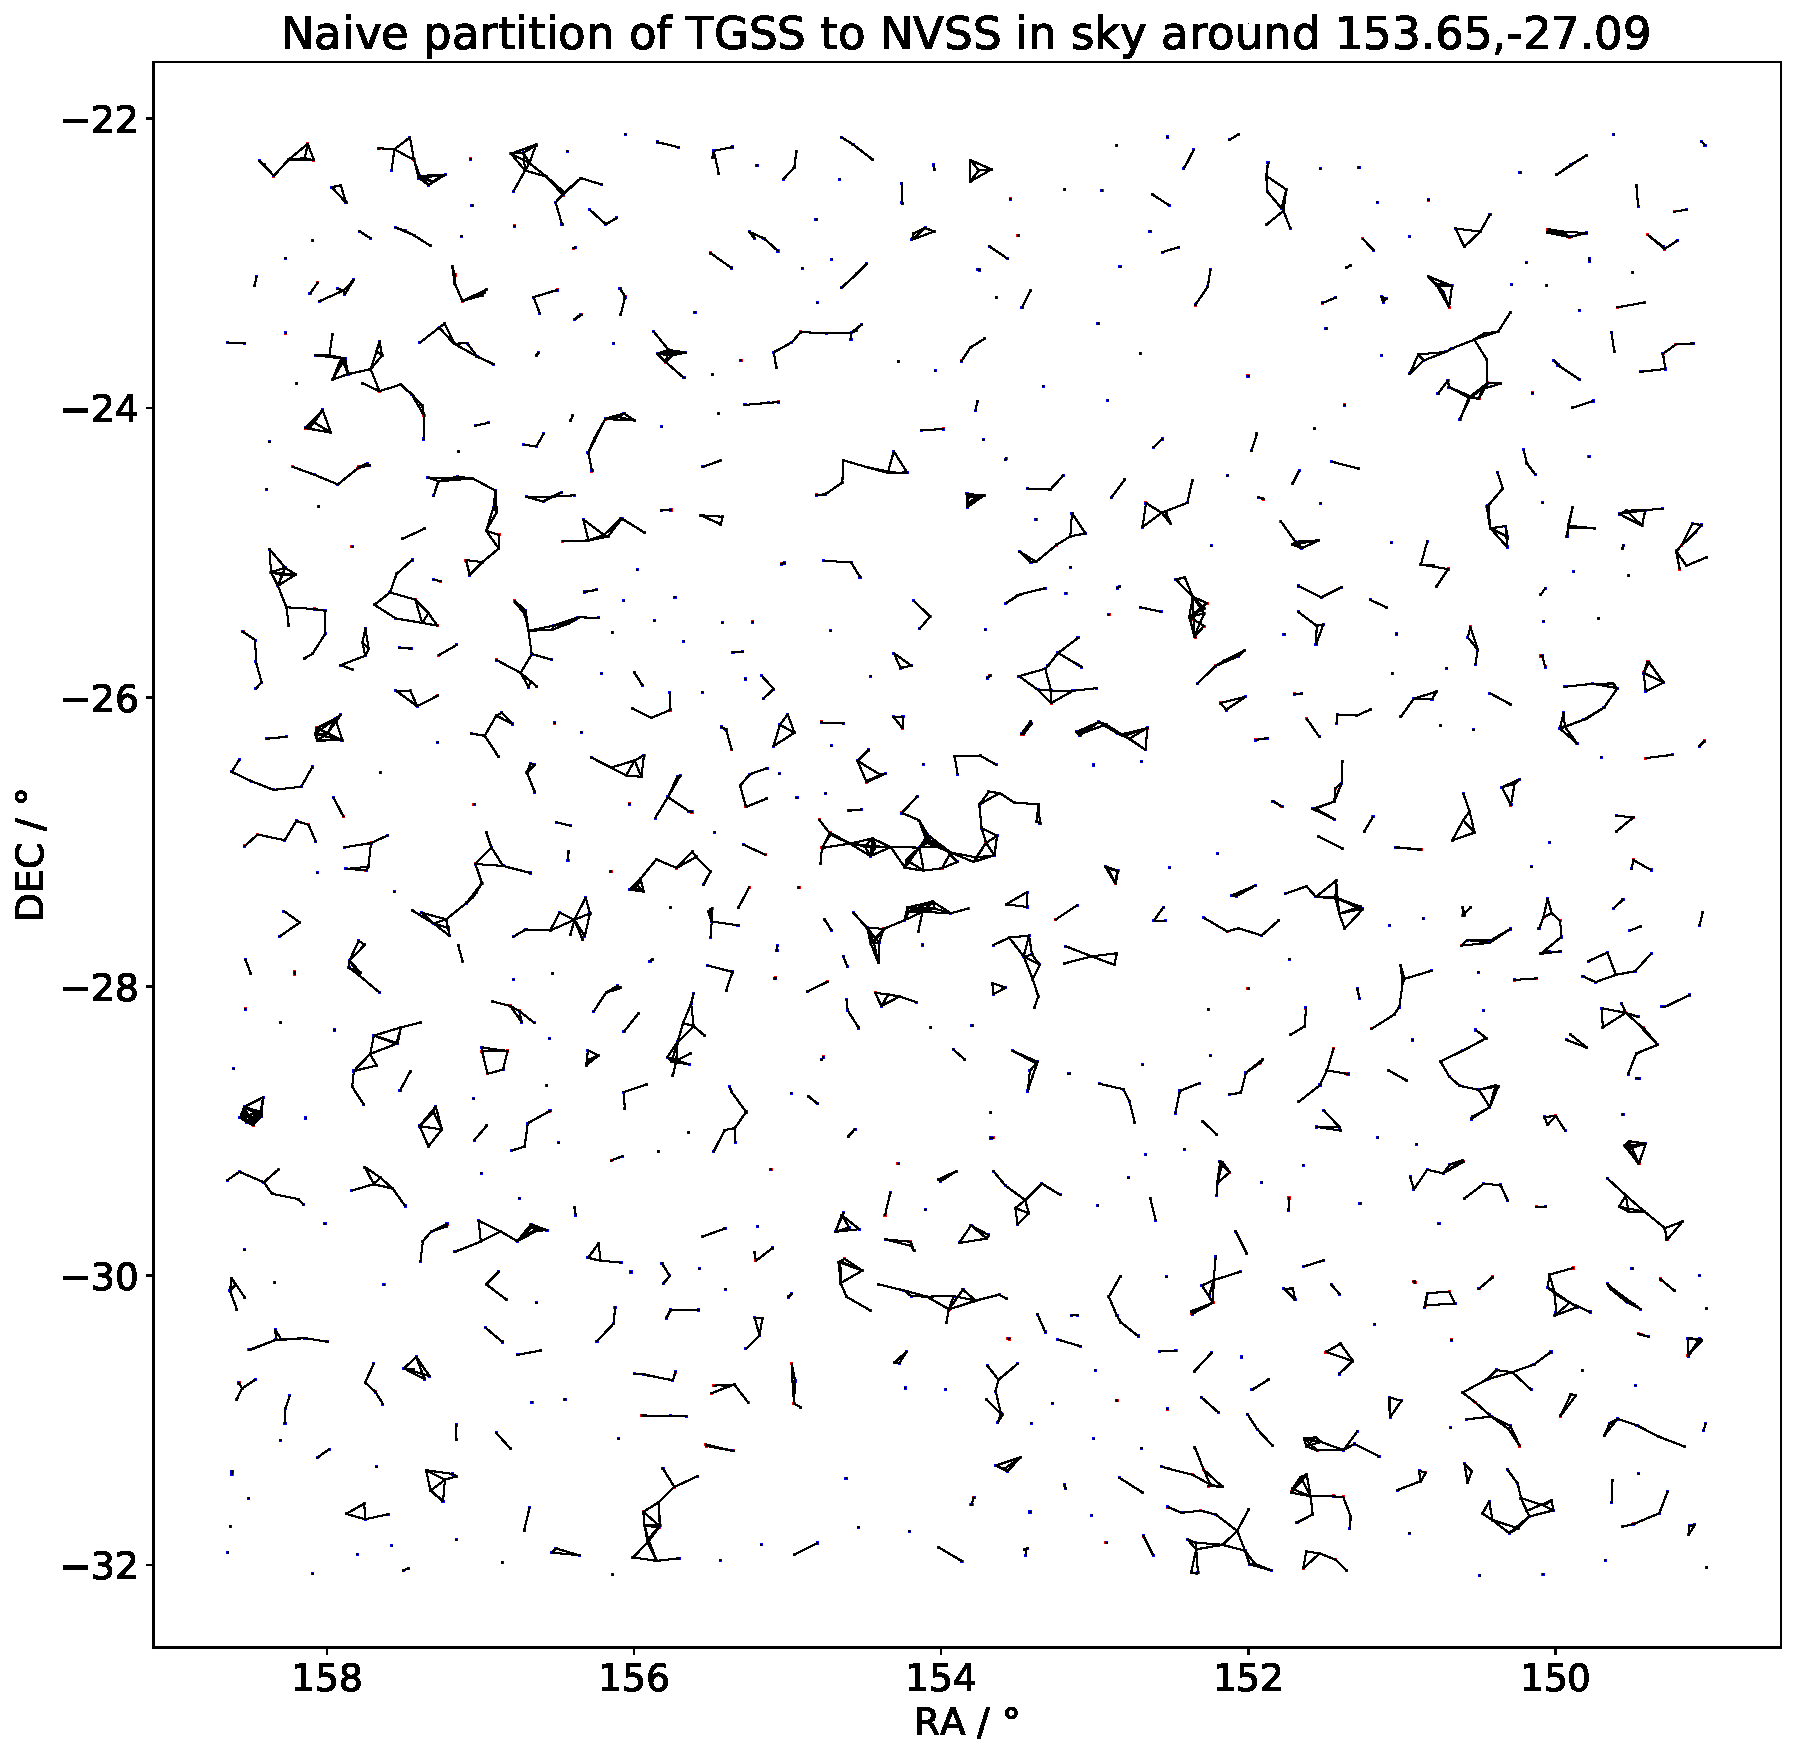
\includegraphics[width=\textwidth]{pics/torch_lr_partition.pdf}
    \caption{Naive partition of the sky using classifier: naive partition aggregates matches transitively, i.e. if T1 matches N1 matches T2 then (T1,N1,T2) forms an object on the sky and the two T-N (TGSS to NVSS) matches are filled in as line segments on the sky. Note how this leads to large (compared to 40') `constellations' on the sky, almost all of which are thought to be unphysical. It also still leads to 1-to-1 matches, which just appear as dots, when nothing else is nearby.}
    \label{fig:torch_lr_partition}%snowflake
\end{figure}

\begin{figure}[ht]
    \centering
    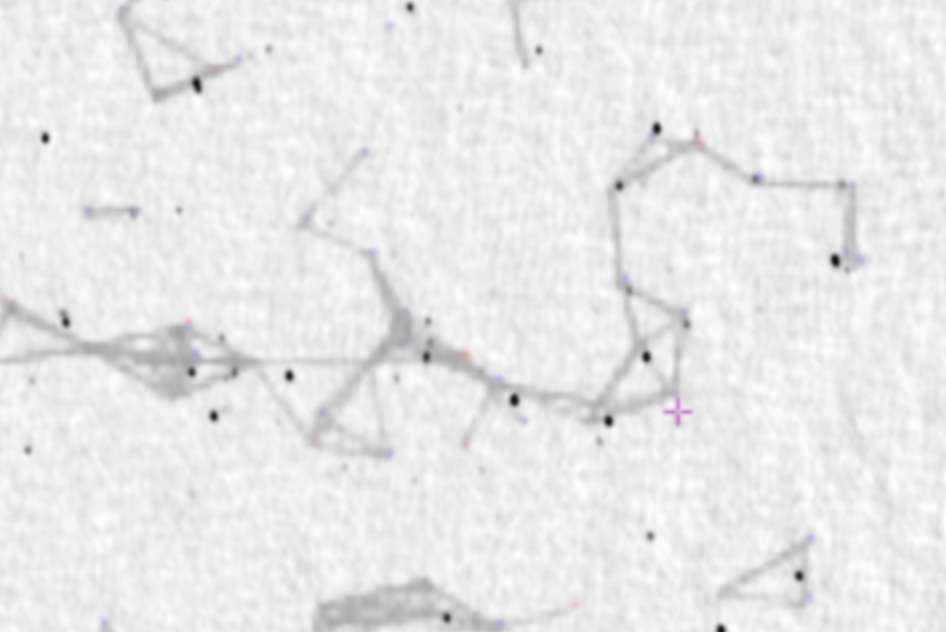
\includegraphics[width=0.6\textwidth]{pics/overlayoverlay.png}
    \caption{Overlay of detail from figure~\ref{fig:torch_lr_partition} over TGSS cut-out, not exactly aligned but one can clearly see that the naive transitive partition has clearly linked distinct compact sources together into a many-component, non-existent physical object}
    \label{fig:overlay}
\end{figure}


\newpage
\section{Discussion}


% non transitive partitioning


% wild speculation


\bigskip
\section{Conclusions}
Our goal was to cross-identify TGSS and NVSS as to be able to identify the real, physical objects in the sky. To this end, we constructed a common catalogue of positional matches of TGSS to NVSS sources within $\ang{;2;}$ over the shared sky and successfully reproduced the initial results of \citet{posmatchpaper}.\\

We then restated the problem as a binary classification task and trained a logistic regression classifier against positional matching labels. This classifier successfully predicted positional matching and manual labels, both with and without the separation feature.\\

Finally, we used the classifier to perform a naive transitive partition of the sky into predicted physical objects. This partition did not appear remotely physical. We find the fault to lie with naive transitive partitioning, positional matching, and not with the classifier.

\bigskip
\nocite{*}
\bibliographystyle{plainnat}
\bibliography{refs}
% - - - - - - - - - - - - - - - - - - - - - - - - - - - -

\newpage
\section{Appendices}
\subsection{Artefact README.txt excerpt}
\label{app:artefact}
Current build found at:
\url{https://github.com/MatthewJA/blobmatch}

TGSS and NVSS radio object surveys available from:\\
\url{https://github.com/MatthewJA/blobmatch/releases/download/v0.1/TGSSADR1_7sigma_catalog.tsv.gz}\\
\url{https://github.com/MatthewJA/blobmatch/releases/download/v0.1/CATALOG.FIT.gz}

\begin{verbatim}
Directory structure:
blobmatch/
    source/
        (all .ipynb notebooks, manual_labels.csv)
    report/
        pics/
            (all plots as .pdf saved by above
            notebooks, also cut-out comparison)
        main.tex
        report.pdf
    project/
        (non-plot outputs of notebooks except
        sky_matches.csv and sky_catalogue.csv,
        also defunct scipts and plots)
    README.txt
    LICENSE
    .gitignore
\end{verbatim}

blobmatch/source/ .ipynb notebooks:
\begin{itemize}
    \item feature\_vectors.ipynb\\
(constructs feature vectors from source catalogues in a patch, labels based off of positional matching)

    \item torch\_logistic\_regression.ipynb\\
(performs logistic regression using pytorch, partitions sky into physical objects)

    \item sklearn\_logistic\_regression.ipynb\\
(performs logistic regression and random forest using sklearn)

    \item score\_feature\_vectors.ipynb\\
(scores the match feature vectors in patch against various metrics, finds each individual source's best match)

    \item sky\_positional\_matching.ipynb\\
(constructs catalogue of primitive feature vectors over entire sky in catalogues, performs positional matching)
\end{itemize}

\subsection{Loss curve}
\label{app:losses}
% torch_lr_losses_nosep
\begin{figure}[H]
    \centering
    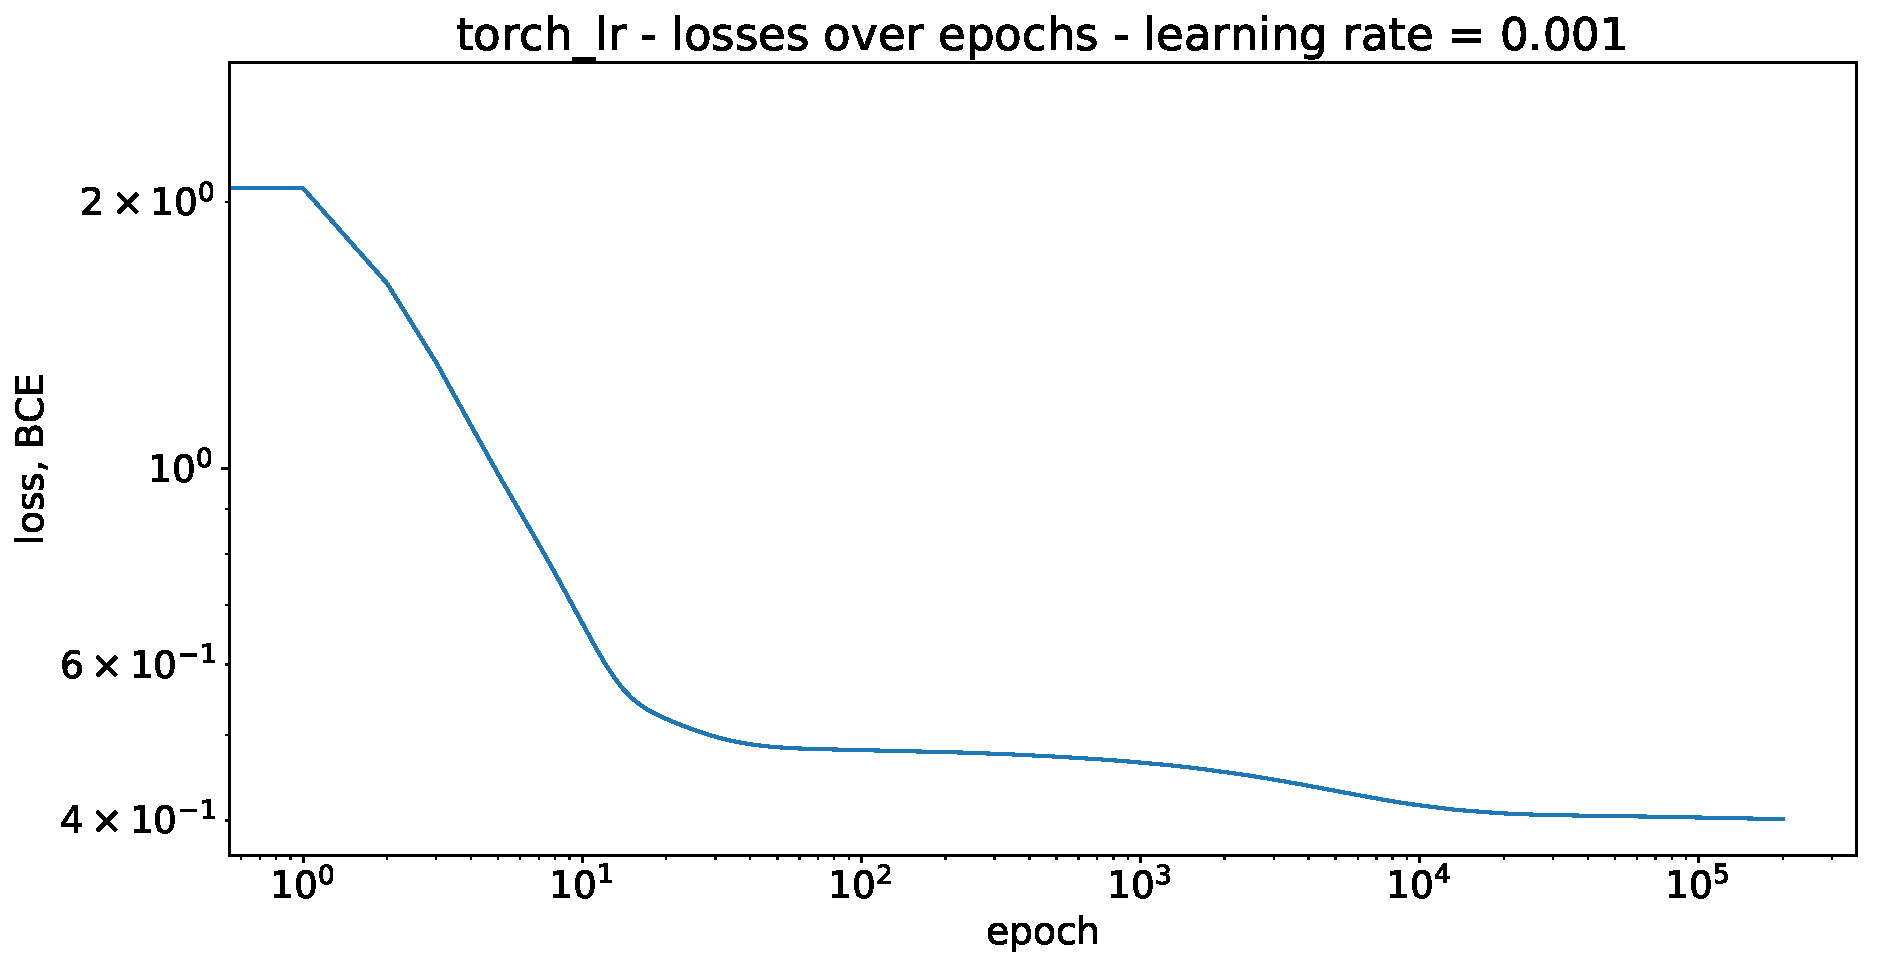
\includegraphics[width=\textwidth]{pics/torch_lr_losses_nosep.pdf}
    \caption{Loss curve for pytorch logistic regression without separation, note the stabilisation after 1e5 epochs of training, we can be hopeful that we've reached some local minimum}
    \label{fig:torch_lr_losses_nosep}
\end{figure}

\subsection{Scikit-learn}
\label{app:sklearn}

We also ran logistic regression through scikit-learn~\citep{sklearn}, this proved both faster and more accurate than the pytorch model. See table~\ref{tab:accuracy} for accuracy.

% sklearn_lr
\begin{figure}[H]
    \centering
    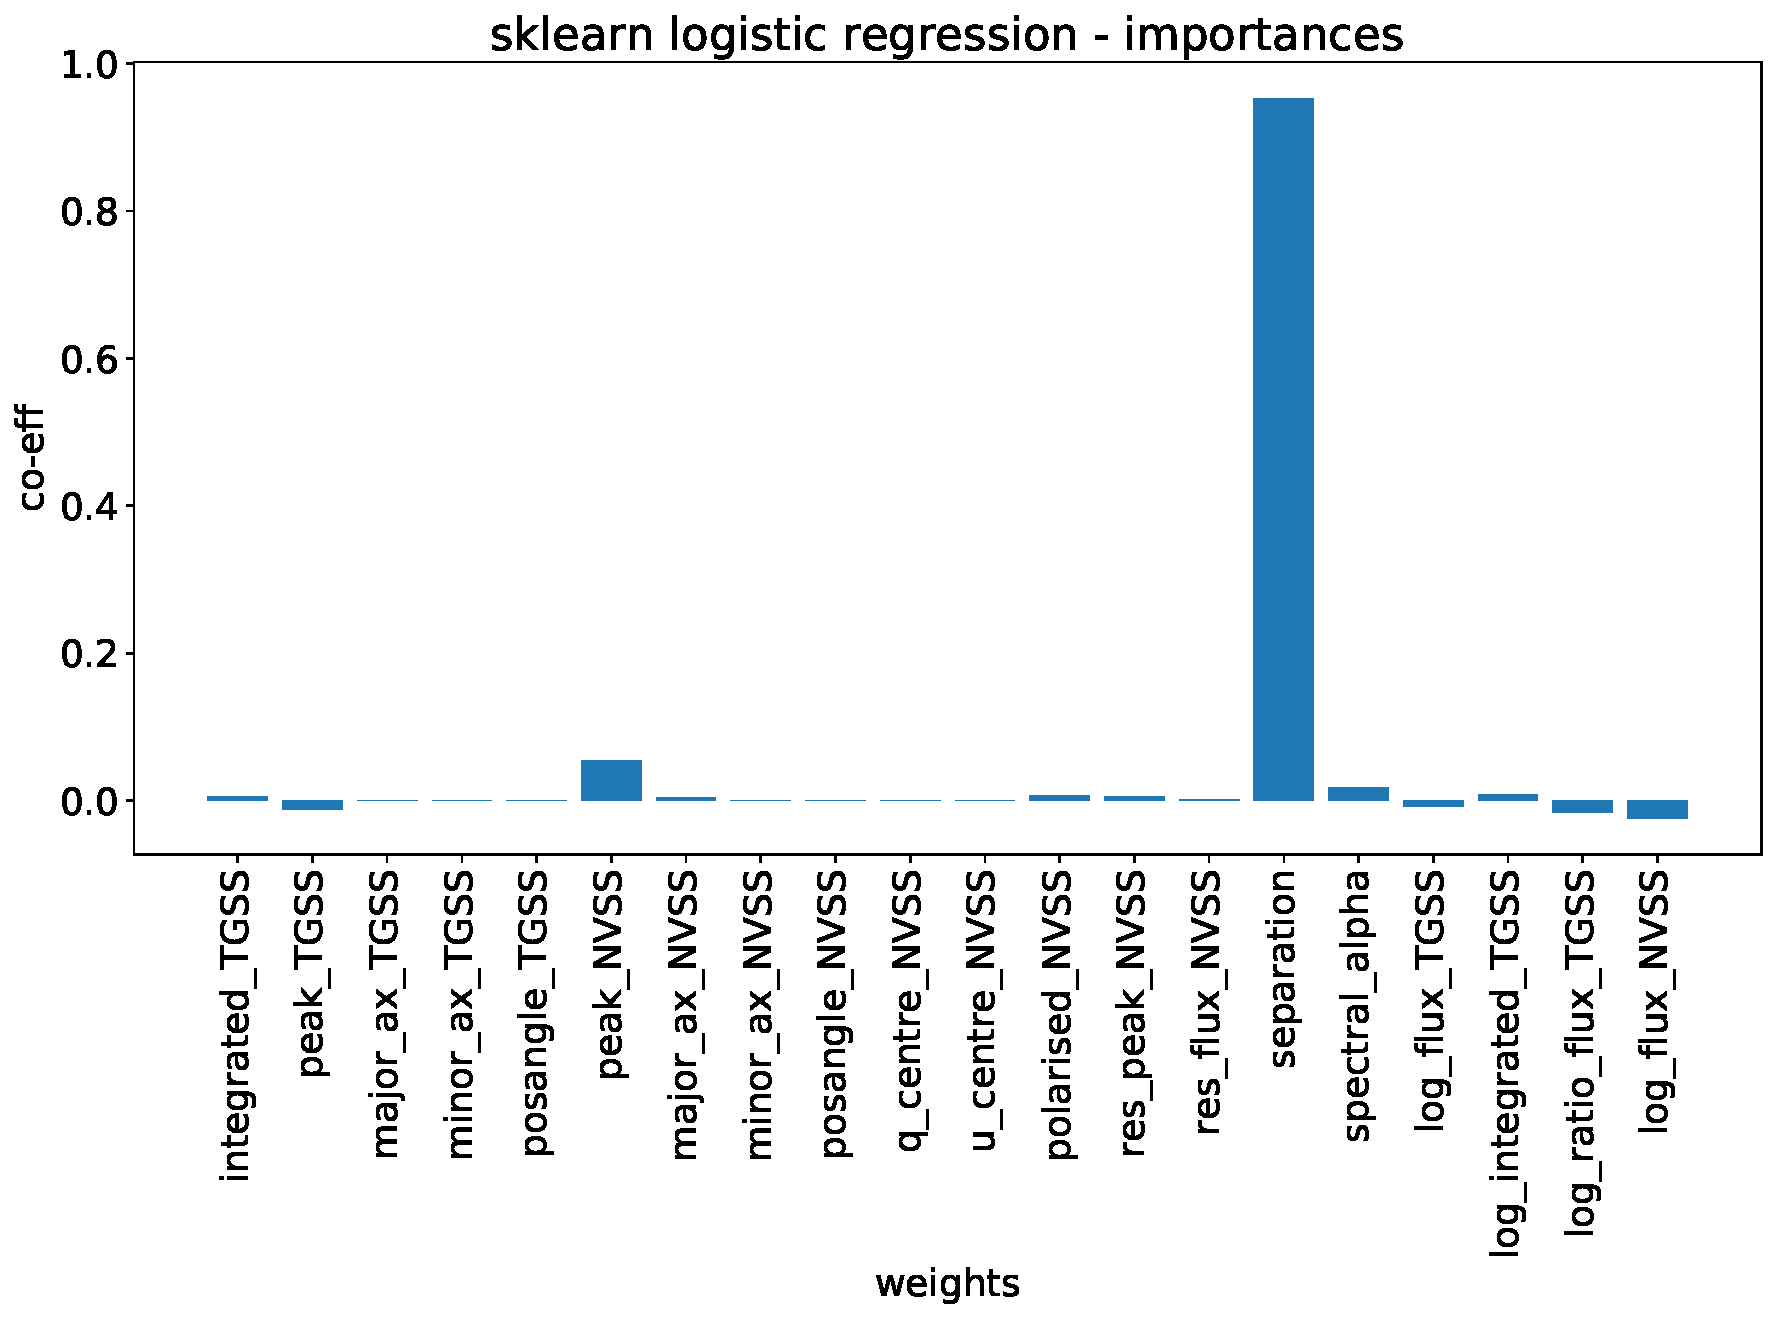
\includegraphics[width=\textwidth]{pics/sklearn_lr.pdf}
    \caption{Logistic regression weights (importances) from scikit-learn model}
    \label{fig:sklearn_lr}
\end{figure}

\subsection{TGSS-NVSS view on partition}
\label{app:windows}

% tgss_window, nvss_window
\begin{figure}[H]
    \begin{subfigure}{1\textwidth}
        \centering
        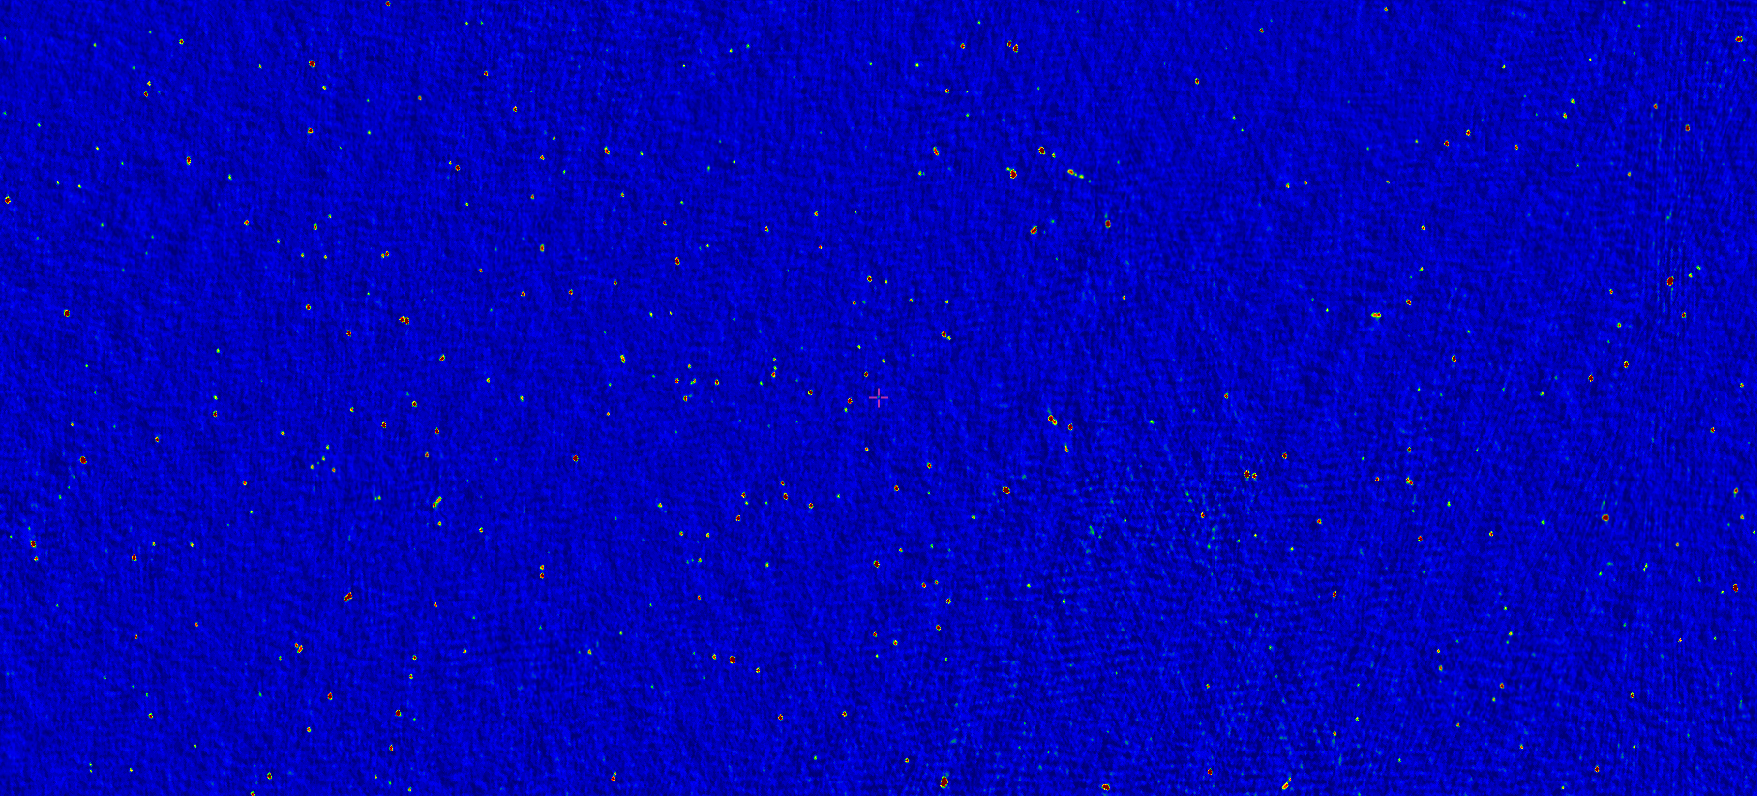
\includegraphics[width=1\linewidth]{pics/tgss_window.pdf}
        % \caption{Put your sub-caption here}
        \label{fig:tgss_window} 
    \end{subfigure}
    \\
    \begin{subfigure}{1\textwidth}
      \centering
        % include second image
        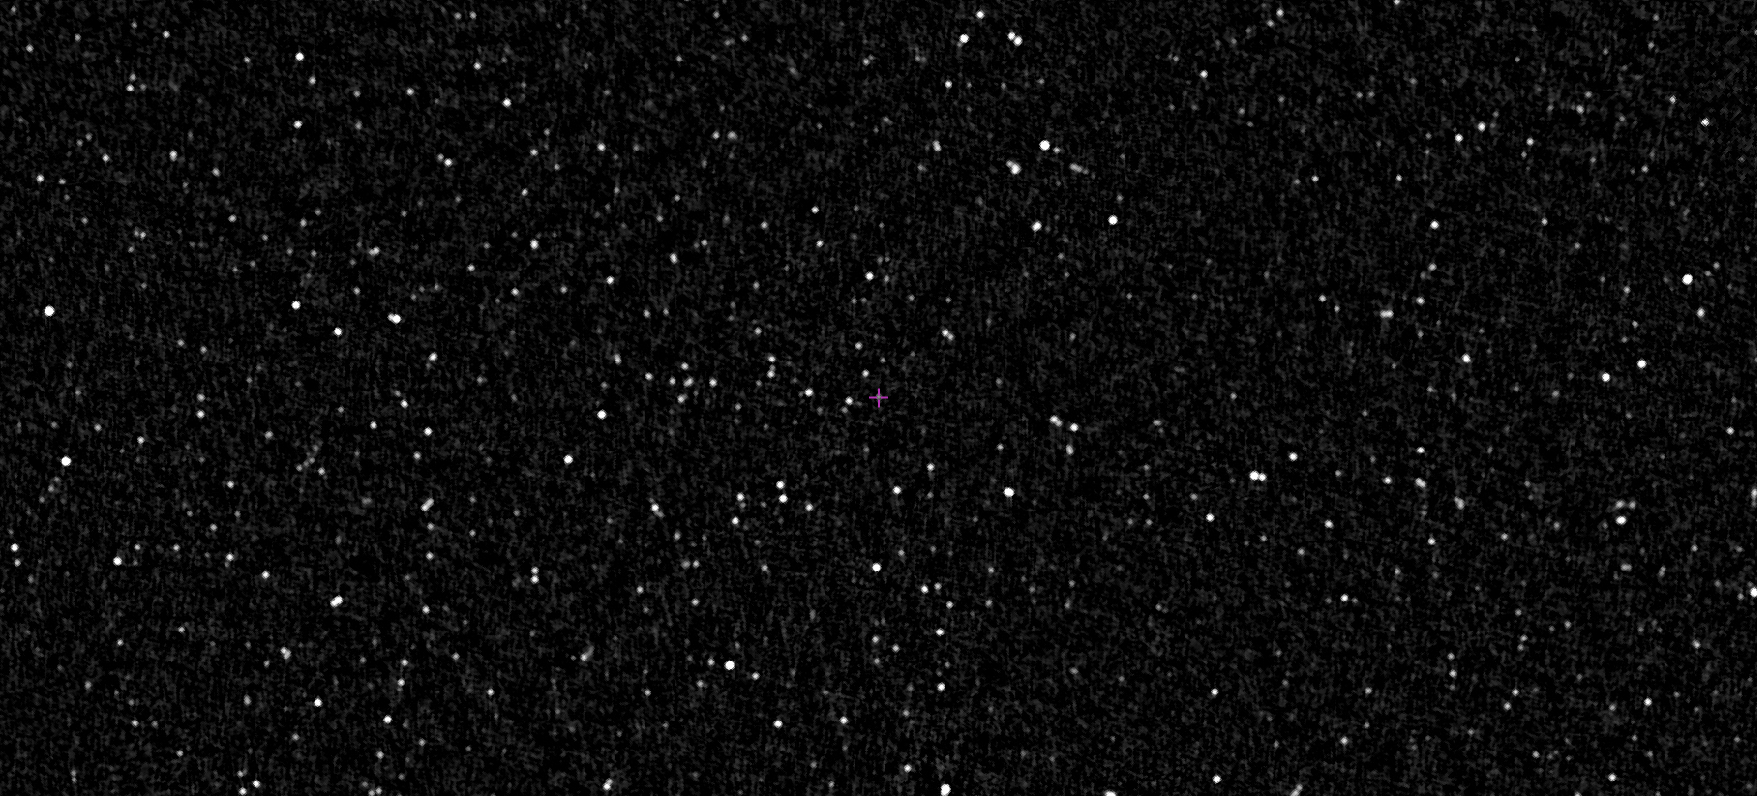
\includegraphics[width=1\linewidth]{pics/nvss_window.pdf}
        % \caption{Put your sub-caption here}
        \label{fig:sub-nvss_window}
    \end{subfigure}
    \caption{Cut-outs of TGSS and NVSS over the partitioned patch of sky shown in
    figure~\ref{fig:torch_lr_partition}, taken from AladinLite~\citep{aladinlite} in 5 degree window around  J101436.8-270532}
    \label{fig:tgss-nvss-windows}
\end{figure}


\end{document}
% - - - - - - - - - - - - - - - - - - - - 
